% **************************************************************************************************************
% A Classic Thesis Style
% An Homage to The Elements of Typographic Style
%
% Copyright (C) 2015 André Miede http://www.miede.de
%
% If you like the style then I would appreciate a postcard. My address 
% can be found in the file ClassicThesis.pdf. A collection of the 
% postcards I received so far is available online at 
% http://postcards.miede.de
%
% License:
% This program is free software; you can redistribute it and/or modify
% it under the terms of the GNU General Public License as published by
% the Free Software Foundation; either version 2 of the License, or
% (at your option) any later version.
%
% This program is distributed in the hope that it will be useful,
% but WITHOUT ANY WARRANTY; without even the implied warranty of
% MERCHANTABILITY or FITNESS FOR A PARTICULAR PURPOSE.  See the
% GNU General Public License for more details.
%
% You should have received a copy of the GNU General Public License
% along with this program; see the file COPYING.  If not, write to
% the Free Software Foundation, Inc., 59 Temple Place - Suite 330,
% Boston, MA 02111-1307, USA.
%
% **************************************************************************************************************
\RequirePackage{fix-cm} % fix some latex issues see: http://texdoc.net/texmf-dist/doc/latex/base/fixltx2e.pdf
\documentclass[ twoside,openright,titlepage,numbers=noenddot,headinclude,%1headlines,% letterpaper a4paper
                footinclude=true,cleardoublepage=empty,abstractoff, % <--- obsolete, remove (todo)
                BCOR=5mm,paper=a4,fontsize=11pt,%11pt,a4paper,%
                ngerman,american,%
                ]{scrreprt}

% ****************************************************************************************************
% Set the encoding of your files. UTF-8 is the only sensible encoding nowadays. If you can't read
% äöüßáéçèê∂åëæƒÏ€ then change the encoding setting in your editor, not the line below. If your editor
% does not support utf8 use another editor!
% ****************************************************************************************************
\PassOptionsToPackage{utf8}{inputenc}
	\usepackage{inputenc}
	
\usepackage{etoolbox}

% ****************************************************************************************************
% Insert the information about your thesis here
% ****************************************************************************************************
\newcommand{\myTitle}{AnSiAn - Android Signal Analyzer\xspace}
\newcommand{\myDegree}{Secure Mobile Networking Project Documentation\xspace}
\newcommand{\myName}{Matthias Kannwischer\xspace}
\newcommand{\myProf}{Prof. Dr.-Ing. Matthias Hollick\xspace}
%\newcommand{\myOtherProf}{Second advisor\xspace}
\newcommand{\mySupervisor}{Jiska Classen\xspace}
\newcommand{\myFaculty}{Department of Computer Science\xspace}
\newcommand{\myDepartment}{Secure Mobile Networking Lab\xspace}
\newcommand{\myUni}{\protect{Technische Universität Darmstadt}\xspace}
\newcommand{\myLocation}{Darmstadt\xspace}
\newcommand{\myTime}{\formatdate{09}{03}{2017}\xspace}
\newcommand{\myVersion}{0.1\xspace}

% Choose if you want the standard template with enough space for margin notes or the tempate with small margins
\newtoggle{adrianstyle}
%\toggletrue{adrianstyle} % uncomment this line to have smaller margins
\togglefalse{adrianstyle} % uncomment this line for the standard seemoo template

%********************************************************************
% Note: Make all your adjustments in here
%*******************************************************
% ****************************************************************************************************
% classicthesis-config.tex 
% formerly known as loadpackages.sty, classicthesis-ldpkg.sty, and classicthesis-preamble.sty 
% Use it at the beginning of your ClassicThesis.tex, or as a LaTeX Preamble 
% in your ClassicThesis.{tex,lyx} with % ****************************************************************************************************
% classicthesis-config.tex 
% formerly known as loadpackages.sty, classicthesis-ldpkg.sty, and classicthesis-preamble.sty 
% Use it at the beginning of your ClassicThesis.tex, or as a LaTeX Preamble 
% in your ClassicThesis.{tex,lyx} with % ****************************************************************************************************
% classicthesis-config.tex 
% formerly known as loadpackages.sty, classicthesis-ldpkg.sty, and classicthesis-preamble.sty 
% Use it at the beginning of your ClassicThesis.tex, or as a LaTeX Preamble 
% in your ClassicThesis.{tex,lyx} with \input{classicthesis-config}
% ****************************************************************************************************  
% If you like the classicthesis, then I would appreciate a postcard. 
% My address can be found in the file ClassicThesis.pdf. A collection 
% of the postcards I received so far is available online at 
% http://postcards.miede.de
% ****************************************************************************************************

% ****************************************************************************************************
% 1. Configure classicthesis for your needs here, e.g., remove "drafting" below 
% in order to deactivate the time-stamp on the pages
% ****************************************************************************************************
\PassOptionsToPackage{eulerchapternumbers,listings,%
                 %drafting,%
				 pdfspacing,%floatperchapter,%linedheaders,%
				 subfig,beramono,eulermath,parts,dottedtoc,%
				 \iftoggle{adrianstyle}{adrianstyle}{}, % Use this option to increase the text width
				 }{classicthesis}								
% ********************************************************************
% Available options for classicthesis.sty 
% (see ClassicThesis.pdf for more information):
% drafting
% parts nochapters linedheaders
% eulerchapternumbers beramono eulermath pdfspacing minionprospacing
% tocaligned dottedtoc manychapters
% listings floatperchapter subfig
% ********************************************************************


% ****************************************************************************************************
% 2. Loading some handy packages
% ****************************************************************************************************
%\PassOptionsToPackage{spanish,es-lcroman}{babel}

% ********************************************************************
% Setup, finetuning, and useful commands
% ********************************************************************
\newcounter{dummy} % necessary for correct hyperlinks (to index, bib, etc.)
\newlength{\abcd} % for ab..z string length calculation
% ****************************************************************************************************


% ****************************************************************************************************
% 3. Loading some handy packages
% ****************************************************************************************************
% ******************************************************************** 
% Packages with options that might require adjustments
% ******************************************************************** 
%\PassOptionsToPackage{ngerman,american}{babel}   % change this to your language(s)
% Spanish languages need extra options in order to work with this template
%\PassOptionsToPackage{spanish,es-lcroman}{babel}
	\usepackage{babel}                  

\usepackage{csquotes}
\PassOptionsToPackage{%
    %backend=biber, %instead of bibtex
	backend=bibtex8,bibencoding=ascii,%
	language=auto,%
	style=numeric-comp,%
    %style=authoryear-comp, % Author 1999, 2010
    %bibstyle=authoryear,dashed=false, % dashed: substitute rep. author with ---
    sorting=nyt, % name, year, title
    maxbibnames=10, % default: 3, et al.
    %backref=true,%
    natbib=true % natbib compatibility mode (\citep and \citet still work)
}{biblatex}
    \usepackage{biblatex}

\PassOptionsToPackage{fleqn}{amsmath}       % math environments and more by the AMS 
    \usepackage{amsmath}

% ******************************************************************** 
% General useful packages
% ******************************************************************** 
\PassOptionsToPackage{T1}{fontenc} % T2A for cyrillics
    \usepackage{fontenc}     
\usepackage{textcomp} % fix warning with missing font shapes
\usepackage{scrhack} % fix warnings when using KOMA with listings package          
\usepackage{xspace} % to get the spacing after macros right  
\usepackage{mparhack} % get marginpar right
\usepackage{fixltx2e} % fixes some LaTeX stuff --> since 2015 in the LaTeX kernel (see below)
\usepackage{acronym}
%\usepackage[latest]{latexrelease} % will be used once available in more distributions (ISSUE #107)
%\usepackage[nopostdot,acronym,shortcuts,nonumberlist]{glossaries}
%\makeglossaries
%\renewcommand*{\glossarysection}[2][]{}
%\input{acronyms.tex}

% ****************************************************************************************************


% ****************************************************************************************************
% 4. Setup floats: tables, (sub)figures, and captions
% ****************************************************************************************************
\usepackage{tabularx} % better tables
    \setlength{\extrarowheight}{3pt} % increase table row height
\newcommand{\tableheadline}[1]{\multicolumn{1}{c}{\spacedlowsmallcaps{#1}}}
\newcommand{\myfloatalign}{\centering} % to be used with each float for alignment
\usepackage{caption}
% Thanks to cgnieder and Claus Lahiri
% http://tex.stackexchange.com/questions/69349/spacedlowsmallcaps-in-caption-label
% [REMOVED DUE TO OTHER PROBLEMS, SEE ISSUE #82]    
%\DeclareCaptionLabelFormat{smallcaps}{\bothIfFirst{#1}{~}\MakeTextLowercase{\textsc{#2}}}
%\captionsetup{font=small,labelformat=smallcaps} % format=hang,
\captionsetup{font=small} % format=hang,
\usepackage{subfig}  
% ****************************************************************************************************


% ****************************************************************************************************
% 5. Setup code listings
% ****************************************************************************************************
\usepackage{listings} 
%\lstset{emph={trueIndex,root},emphstyle=\color{BlueViolet}}%\underbar} % for special keywords
\lstset{language=[LaTeX]Tex,%C++,
    morekeywords={PassOptionsToPackage,selectlanguage},
    keywordstyle=\color{RoyalBlue},%\bfseries,
    basicstyle=\small\ttfamily,
    %identifierstyle=\color{NavyBlue},
    commentstyle=\color{Green}\ttfamily,
    stringstyle=\rmfamily,
    numbers=none,%left,%
    numberstyle=\scriptsize,%\tiny
    stepnumber=5,
    numbersep=8pt,
    showstringspaces=false,
    breaklines=true,
    %frameround=ftff,
    %frame=single,
    belowcaptionskip=.75\baselineskip
    %frame=L
} 
% ****************************************************************************************************    		   


% ****************************************************************************************************
% 6. PDFLaTeX, hyperreferences and citation backreferences
% ****************************************************************************************************
% ********************************************************************
% Using PDFLaTeX
% ********************************************************************
\PassOptionsToPackage{pdftex,hyperfootnotes=false,pdfpagelabels}{hyperref}
    \usepackage{hyperref}  % backref linktocpage pagebackref
\pdfcompresslevel=9
\pdfadjustspacing=1 
\PassOptionsToPackage{pdftex}{graphicx}
    \usepackage{graphicx} 
 

% ********************************************************************
% Hyperreferences
% ********************************************************************
\hypersetup{%
    %draft,	% = no hyperlinking at all (useful in b/w printouts)
    %colorlinks=true, linktocpage=true, pdfstartpage=3, pdfstartview=FitV,%
    % uncomment the following line if you want to have black links (e.g., for printing)
    colorlinks=false, linktocpage=false, pdfborder={0 0 0}, pdfstartpage=3, pdfstartview=FitV,% 
    breaklinks=true, pdfpagemode=UseNone, pageanchor=true, pdfpagemode=UseOutlines,%
    plainpages=false, bookmarksnumbered, bookmarksopen=true, bookmarksopenlevel=1,%
    hypertexnames=true, pdfhighlight=/O,%nesting=true,%frenchlinks,%
    urlcolor=webbrown, linkcolor=RoyalBlue, citecolor=webgreen, %pagecolor=RoyalBlue,%
    %urlcolor=Black, linkcolor=Black, citecolor=Black, %pagecolor=Black,%
    pdftitle={\myTitle},%
    pdfauthor={\textcopyright\ \myName, \myUni, \myFaculty},%
    pdfsubject={},%
    pdfkeywords={},%
    pdfcreator={pdfLaTeX},%
    pdfproducer={LaTeX with hyperref and classicthesis}%
}

\pdfinfo{
   /CreationDate (D:20130424083342)
   /ModDate (D:20130424083342)
}

% ********************************************************************
% Setup autoreferences
% ********************************************************************
% There are some issues regarding autorefnames
% http://www.ureader.de/msg/136221647.aspx
% http://www.tex.ac.uk/cgi-bin/texfaq2html?label=latexwords
% you have to redefine the makros for the 
% language you use, e.g., american, ngerman
% (as chosen when loading babel/AtBeginDocument)
% ********************************************************************
\makeatletter
\@ifpackageloaded{babel}%
    {%
       \addto\extrasamerican{%
			\renewcommand*{\figureautorefname}{Figure}%
			\renewcommand*{\tableautorefname}{Table}%
			\renewcommand*{\partautorefname}{Part}%
			\renewcommand*{\chapterautorefname}{Chapter}%
			\renewcommand*{\sectionautorefname}{Section}%
			\renewcommand*{\subsectionautorefname}{Section}%
			\renewcommand*{\subsubsectionautorefname}{Section}%     
                }%
       \addto\extrasngerman{% 
			\renewcommand*{\paragraphautorefname}{Absatz}%
			\renewcommand*{\subparagraphautorefname}{Unterabsatz}%
			\renewcommand*{\footnoteautorefname}{Fu\"snote}%
			\renewcommand*{\FancyVerbLineautorefname}{Zeile}%
			\renewcommand*{\theoremautorefname}{Theorem}%
			\renewcommand*{\appendixautorefname}{Anhang}%
			\renewcommand*{\equationautorefname}{Gleichung}%        
			\renewcommand*{\itemautorefname}{Punkt}%
                }%  
            % Fix to getting autorefs for subfigures right (thanks to Belinda Vogt for changing the definition)
            \providecommand{\subfigureautorefname}{\figureautorefname}%             
    }{\relax}
\makeatother


% ****************************************************************************************************
% 7. Last calls before the bar closes
% ****************************************************************************************************
% ********************************************************************
% Development Stuff
% ********************************************************************
\listfiles
%\PassOptionsToPackage{l2tabu,orthodox,abort}{nag}
%   \usepackage{nag}
%\PassOptionsToPackage{warning, all}{onlyamsmath}
%   \usepackage{onlyamsmath}

% ********************************************************************
% Last, but not least...
% ********************************************************************
\usepackage{classicthesis} 
% ****************************************************************************************************


% ****************************************************************************************************
% 8. Further adjustments (experimental)
% ****************************************************************************************************
% ********************************************************************
% Changing the text area
% ********************************************************************
%\linespread{1.05} % a bit more for Palatino
%\areaset[current]{312pt}{761pt} % 686 (factor 2.2) + 33 head + 42 head \the\footskip
%\setlength{\marginparwidth}{7em}%
%\setlength{\marginparsep}{2em}%

% ********************************************************************
% Using different fonts
% ********************************************************************
%\usepackage[oldstylenums]{kpfonts} % oldstyle notextcomp
%\usepackage[osf]{libertine}
%\usepackage[light,condensed,math]{iwona}
%\renewcommand{\sfdefault}{iwona}
%\usepackage{lmodern} % <-- no osf support :-(
%\usepackage{cfr-lm} % 
%\usepackage[urw-garamond]{mathdesign} <-- no osf support :-(
%\usepackage[default,osfigures]{opensans} % scale=0.95 
%\usepackage[sfdefault]{FiraSans}
% ****************************************************************************************************

% ****************************************************************************************************  
% If you like the classicthesis, then I would appreciate a postcard. 
% My address can be found in the file ClassicThesis.pdf. A collection 
% of the postcards I received so far is available online at 
% http://postcards.miede.de
% ****************************************************************************************************

% ****************************************************************************************************
% 1. Configure classicthesis for your needs here, e.g., remove "drafting" below 
% in order to deactivate the time-stamp on the pages
% ****************************************************************************************************
\PassOptionsToPackage{eulerchapternumbers,listings,%
                 %drafting,%
				 pdfspacing,%floatperchapter,%linedheaders,%
				 subfig,beramono,eulermath,parts,dottedtoc,%
				 \iftoggle{adrianstyle}{adrianstyle}{}, % Use this option to increase the text width
				 }{classicthesis}								
% ********************************************************************
% Available options for classicthesis.sty 
% (see ClassicThesis.pdf for more information):
% drafting
% parts nochapters linedheaders
% eulerchapternumbers beramono eulermath pdfspacing minionprospacing
% tocaligned dottedtoc manychapters
% listings floatperchapter subfig
% ********************************************************************


% ****************************************************************************************************
% 2. Loading some handy packages
% ****************************************************************************************************
%\PassOptionsToPackage{spanish,es-lcroman}{babel}

% ********************************************************************
% Setup, finetuning, and useful commands
% ********************************************************************
\newcounter{dummy} % necessary for correct hyperlinks (to index, bib, etc.)
\newlength{\abcd} % for ab..z string length calculation
% ****************************************************************************************************


% ****************************************************************************************************
% 3. Loading some handy packages
% ****************************************************************************************************
% ******************************************************************** 
% Packages with options that might require adjustments
% ******************************************************************** 
%\PassOptionsToPackage{ngerman,american}{babel}   % change this to your language(s)
% Spanish languages need extra options in order to work with this template
%\PassOptionsToPackage{spanish,es-lcroman}{babel}
	\usepackage{babel}                  

\usepackage{csquotes}
\PassOptionsToPackage{%
    %backend=biber, %instead of bibtex
	backend=bibtex8,bibencoding=ascii,%
	language=auto,%
	style=numeric-comp,%
    %style=authoryear-comp, % Author 1999, 2010
    %bibstyle=authoryear,dashed=false, % dashed: substitute rep. author with ---
    sorting=nyt, % name, year, title
    maxbibnames=10, % default: 3, et al.
    %backref=true,%
    natbib=true % natbib compatibility mode (\citep and \citet still work)
}{biblatex}
    \usepackage{biblatex}

\PassOptionsToPackage{fleqn}{amsmath}       % math environments and more by the AMS 
    \usepackage{amsmath}

% ******************************************************************** 
% General useful packages
% ******************************************************************** 
\PassOptionsToPackage{T1}{fontenc} % T2A for cyrillics
    \usepackage{fontenc}     
\usepackage{textcomp} % fix warning with missing font shapes
\usepackage{scrhack} % fix warnings when using KOMA with listings package          
\usepackage{xspace} % to get the spacing after macros right  
\usepackage{mparhack} % get marginpar right
\usepackage{fixltx2e} % fixes some LaTeX stuff --> since 2015 in the LaTeX kernel (see below)
\usepackage{acronym}
%\usepackage[latest]{latexrelease} % will be used once available in more distributions (ISSUE #107)
%\usepackage[nopostdot,acronym,shortcuts,nonumberlist]{glossaries}
%\makeglossaries
%\renewcommand*{\glossarysection}[2][]{}
%\newacronym{NIC}{NIC}{network interface card}
\newacronym{EMR}{EMR}{electromagnetic radiation}
\newacronym{NSA}{NSA}{National Security Agency}
\newacronym{PC}{PC}{personal computer}
\newacronym{USRP}{USRP}{Universal Software Radio Peripheral}
\newacronym{SDR}{SDR}{software-defined radio}
\newacronym{FPGA}{FPGA}{field-programmable gate array}
\newacronym{PA}{PA}{power amplifier}
\newacronym{BCI}{BCI}{bulk current injection}
\newacronym{FEC}{FEC}{forward error correction}
\newacronym{IEC}{IEC}{International Electrotechnical Commission}
\newacronym{SFD}{SFD}{start frame delimiter}
\newacronym{MAC}{MAC}{Medium Access Control}
\newacronym{DAC}{DAC}{digital-to-analog converter}
\newacronym{CSMACD}{CSMA/CD}{carrier sense multiple access with collision detection}
\newacronym{CAN}{CAN}{control area network}
\newacronym{CoE}{CoE}{CAN over Ethernet}
\newacronym{RF}{RF}{radio frequency}
\newacronym{FCS}{FCS}{frame check sum}
\newacronym{ADC}{ADC}{analog-to-digital converter}
\newacronym{(S+N)/NR}{(S+N)/NR}{signal-plus-noise-to-noise ratio}
\newacronym{ICMP}{ICMP}{Internet control message protocol}
\newacronym{DoS}{DoS}{denial of service}
\newacronym{CRT}{CRT}{cathode ray tube}
\newacronym{SNR}{SNR}{signal-to-noise ratio}

\newacronym{AnSiAn}{AnSiAn}{Android Signal Analyzer}
\newacronym{RDS}{RDS}{Radio Data System}
\newacronym{BPSK}{BPSK}{Binary Phase Shift Keying}
\newacronym{QAM}{QAM}{Quadrature amplitude modulation}
\newacronym{FM}{FM}{Frequency Modulation}

% ****************************************************************************************************


% ****************************************************************************************************
% 4. Setup floats: tables, (sub)figures, and captions
% ****************************************************************************************************
\usepackage{tabularx} % better tables
    \setlength{\extrarowheight}{3pt} % increase table row height
\newcommand{\tableheadline}[1]{\multicolumn{1}{c}{\spacedlowsmallcaps{#1}}}
\newcommand{\myfloatalign}{\centering} % to be used with each float for alignment
\usepackage{caption}
% Thanks to cgnieder and Claus Lahiri
% http://tex.stackexchange.com/questions/69349/spacedlowsmallcaps-in-caption-label
% [REMOVED DUE TO OTHER PROBLEMS, SEE ISSUE #82]    
%\DeclareCaptionLabelFormat{smallcaps}{\bothIfFirst{#1}{~}\MakeTextLowercase{\textsc{#2}}}
%\captionsetup{font=small,labelformat=smallcaps} % format=hang,
\captionsetup{font=small} % format=hang,
\usepackage{subfig}  
% ****************************************************************************************************


% ****************************************************************************************************
% 5. Setup code listings
% ****************************************************************************************************
\usepackage{listings} 
%\lstset{emph={trueIndex,root},emphstyle=\color{BlueViolet}}%\underbar} % for special keywords
\lstset{language=[LaTeX]Tex,%C++,
    morekeywords={PassOptionsToPackage,selectlanguage},
    keywordstyle=\color{RoyalBlue},%\bfseries,
    basicstyle=\small\ttfamily,
    %identifierstyle=\color{NavyBlue},
    commentstyle=\color{Green}\ttfamily,
    stringstyle=\rmfamily,
    numbers=none,%left,%
    numberstyle=\scriptsize,%\tiny
    stepnumber=5,
    numbersep=8pt,
    showstringspaces=false,
    breaklines=true,
    %frameround=ftff,
    %frame=single,
    belowcaptionskip=.75\baselineskip
    %frame=L
} 
% ****************************************************************************************************    		   


% ****************************************************************************************************
% 6. PDFLaTeX, hyperreferences and citation backreferences
% ****************************************************************************************************
% ********************************************************************
% Using PDFLaTeX
% ********************************************************************
\PassOptionsToPackage{pdftex,hyperfootnotes=false,pdfpagelabels}{hyperref}
    \usepackage{hyperref}  % backref linktocpage pagebackref
\pdfcompresslevel=9
\pdfadjustspacing=1 
\PassOptionsToPackage{pdftex}{graphicx}
    \usepackage{graphicx} 
 

% ********************************************************************
% Hyperreferences
% ********************************************************************
\hypersetup{%
    %draft,	% = no hyperlinking at all (useful in b/w printouts)
    %colorlinks=true, linktocpage=true, pdfstartpage=3, pdfstartview=FitV,%
    % uncomment the following line if you want to have black links (e.g., for printing)
    colorlinks=false, linktocpage=false, pdfborder={0 0 0}, pdfstartpage=3, pdfstartview=FitV,% 
    breaklinks=true, pdfpagemode=UseNone, pageanchor=true, pdfpagemode=UseOutlines,%
    plainpages=false, bookmarksnumbered, bookmarksopen=true, bookmarksopenlevel=1,%
    hypertexnames=true, pdfhighlight=/O,%nesting=true,%frenchlinks,%
    urlcolor=webbrown, linkcolor=RoyalBlue, citecolor=webgreen, %pagecolor=RoyalBlue,%
    %urlcolor=Black, linkcolor=Black, citecolor=Black, %pagecolor=Black,%
    pdftitle={\myTitle},%
    pdfauthor={\textcopyright\ \myName, \myUni, \myFaculty},%
    pdfsubject={},%
    pdfkeywords={},%
    pdfcreator={pdfLaTeX},%
    pdfproducer={LaTeX with hyperref and classicthesis}%
}

\pdfinfo{
   /CreationDate (D:20130424083342)
   /ModDate (D:20130424083342)
}

% ********************************************************************
% Setup autoreferences
% ********************************************************************
% There are some issues regarding autorefnames
% http://www.ureader.de/msg/136221647.aspx
% http://www.tex.ac.uk/cgi-bin/texfaq2html?label=latexwords
% you have to redefine the makros for the 
% language you use, e.g., american, ngerman
% (as chosen when loading babel/AtBeginDocument)
% ********************************************************************
\makeatletter
\@ifpackageloaded{babel}%
    {%
       \addto\extrasamerican{%
			\renewcommand*{\figureautorefname}{Figure}%
			\renewcommand*{\tableautorefname}{Table}%
			\renewcommand*{\partautorefname}{Part}%
			\renewcommand*{\chapterautorefname}{Chapter}%
			\renewcommand*{\sectionautorefname}{Section}%
			\renewcommand*{\subsectionautorefname}{Section}%
			\renewcommand*{\subsubsectionautorefname}{Section}%     
                }%
       \addto\extrasngerman{% 
			\renewcommand*{\paragraphautorefname}{Absatz}%
			\renewcommand*{\subparagraphautorefname}{Unterabsatz}%
			\renewcommand*{\footnoteautorefname}{Fu\"snote}%
			\renewcommand*{\FancyVerbLineautorefname}{Zeile}%
			\renewcommand*{\theoremautorefname}{Theorem}%
			\renewcommand*{\appendixautorefname}{Anhang}%
			\renewcommand*{\equationautorefname}{Gleichung}%        
			\renewcommand*{\itemautorefname}{Punkt}%
                }%  
            % Fix to getting autorefs for subfigures right (thanks to Belinda Vogt for changing the definition)
            \providecommand{\subfigureautorefname}{\figureautorefname}%             
    }{\relax}
\makeatother


% ****************************************************************************************************
% 7. Last calls before the bar closes
% ****************************************************************************************************
% ********************************************************************
% Development Stuff
% ********************************************************************
\listfiles
%\PassOptionsToPackage{l2tabu,orthodox,abort}{nag}
%   \usepackage{nag}
%\PassOptionsToPackage{warning, all}{onlyamsmath}
%   \usepackage{onlyamsmath}

% ********************************************************************
% Last, but not least...
% ********************************************************************
\usepackage{classicthesis} 
% ****************************************************************************************************


% ****************************************************************************************************
% 8. Further adjustments (experimental)
% ****************************************************************************************************
% ********************************************************************
% Changing the text area
% ********************************************************************
%\linespread{1.05} % a bit more for Palatino
%\areaset[current]{312pt}{761pt} % 686 (factor 2.2) + 33 head + 42 head \the\footskip
%\setlength{\marginparwidth}{7em}%
%\setlength{\marginparsep}{2em}%

% ********************************************************************
% Using different fonts
% ********************************************************************
%\usepackage[oldstylenums]{kpfonts} % oldstyle notextcomp
%\usepackage[osf]{libertine}
%\usepackage[light,condensed,math]{iwona}
%\renewcommand{\sfdefault}{iwona}
%\usepackage{lmodern} % <-- no osf support :-(
%\usepackage{cfr-lm} % 
%\usepackage[urw-garamond]{mathdesign} <-- no osf support :-(
%\usepackage[default,osfigures]{opensans} % scale=0.95 
%\usepackage[sfdefault]{FiraSans}
% ****************************************************************************************************

% ****************************************************************************************************  
% If you like the classicthesis, then I would appreciate a postcard. 
% My address can be found in the file ClassicThesis.pdf. A collection 
% of the postcards I received so far is available online at 
% http://postcards.miede.de
% ****************************************************************************************************

% ****************************************************************************************************
% 1. Configure classicthesis for your needs here, e.g., remove "drafting" below 
% in order to deactivate the time-stamp on the pages
% ****************************************************************************************************
\PassOptionsToPackage{eulerchapternumbers,listings,%
                 %drafting,%
				 pdfspacing,%floatperchapter,%linedheaders,%
				 subfig,beramono,eulermath,parts,dottedtoc,%
				 \iftoggle{adrianstyle}{adrianstyle}{}, % Use this option to increase the text width
				 }{classicthesis}								
% ********************************************************************
% Available options for classicthesis.sty 
% (see ClassicThesis.pdf for more information):
% drafting
% parts nochapters linedheaders
% eulerchapternumbers beramono eulermath pdfspacing minionprospacing
% tocaligned dottedtoc manychapters
% listings floatperchapter subfig
% ********************************************************************


% ****************************************************************************************************
% 2. Loading some handy packages
% ****************************************************************************************************
%\PassOptionsToPackage{spanish,es-lcroman}{babel}

% ********************************************************************
% Setup, finetuning, and useful commands
% ********************************************************************
\newcounter{dummy} % necessary for correct hyperlinks (to index, bib, etc.)
\newlength{\abcd} % for ab..z string length calculation
% ****************************************************************************************************


% ****************************************************************************************************
% 3. Loading some handy packages
% ****************************************************************************************************
% ******************************************************************** 
% Packages with options that might require adjustments
% ******************************************************************** 
%\PassOptionsToPackage{ngerman,american}{babel}   % change this to your language(s)
% Spanish languages need extra options in order to work with this template
%\PassOptionsToPackage{spanish,es-lcroman}{babel}
	\usepackage{babel}                  

\usepackage{csquotes}
\PassOptionsToPackage{%
    %backend=biber, %instead of bibtex
	backend=bibtex8,bibencoding=ascii,%
	language=auto,%
	style=numeric-comp,%
    %style=authoryear-comp, % Author 1999, 2010
    %bibstyle=authoryear,dashed=false, % dashed: substitute rep. author with ---
    sorting=nyt, % name, year, title
    maxbibnames=10, % default: 3, et al.
    %backref=true,%
    natbib=true % natbib compatibility mode (\citep and \citet still work)
}{biblatex}
    \usepackage{biblatex}

\PassOptionsToPackage{fleqn}{amsmath}       % math environments and more by the AMS 
    \usepackage{amsmath}

% ******************************************************************** 
% General useful packages
% ******************************************************************** 
\PassOptionsToPackage{T1}{fontenc} % T2A for cyrillics
    \usepackage{fontenc}     
\usepackage{textcomp} % fix warning with missing font shapes
\usepackage{scrhack} % fix warnings when using KOMA with listings package          
\usepackage{xspace} % to get the spacing after macros right  
\usepackage{mparhack} % get marginpar right
\usepackage{fixltx2e} % fixes some LaTeX stuff --> since 2015 in the LaTeX kernel (see below)
\usepackage{acronym}
%\usepackage[latest]{latexrelease} % will be used once available in more distributions (ISSUE #107)
%\usepackage[nopostdot,acronym,shortcuts,nonumberlist]{glossaries}
%\makeglossaries
%\renewcommand*{\glossarysection}[2][]{}
%\newacronym{NIC}{NIC}{network interface card}
\newacronym{EMR}{EMR}{electromagnetic radiation}
\newacronym{NSA}{NSA}{National Security Agency}
\newacronym{PC}{PC}{personal computer}
\newacronym{USRP}{USRP}{Universal Software Radio Peripheral}
\newacronym{SDR}{SDR}{software-defined radio}
\newacronym{FPGA}{FPGA}{field-programmable gate array}
\newacronym{PA}{PA}{power amplifier}
\newacronym{BCI}{BCI}{bulk current injection}
\newacronym{FEC}{FEC}{forward error correction}
\newacronym{IEC}{IEC}{International Electrotechnical Commission}
\newacronym{SFD}{SFD}{start frame delimiter}
\newacronym{MAC}{MAC}{Medium Access Control}
\newacronym{DAC}{DAC}{digital-to-analog converter}
\newacronym{CSMACD}{CSMA/CD}{carrier sense multiple access with collision detection}
\newacronym{CAN}{CAN}{control area network}
\newacronym{CoE}{CoE}{CAN over Ethernet}
\newacronym{RF}{RF}{radio frequency}
\newacronym{FCS}{FCS}{frame check sum}
\newacronym{ADC}{ADC}{analog-to-digital converter}
\newacronym{(S+N)/NR}{(S+N)/NR}{signal-plus-noise-to-noise ratio}
\newacronym{ICMP}{ICMP}{Internet control message protocol}
\newacronym{DoS}{DoS}{denial of service}
\newacronym{CRT}{CRT}{cathode ray tube}
\newacronym{SNR}{SNR}{signal-to-noise ratio}

\newacronym{AnSiAn}{AnSiAn}{Android Signal Analyzer}
\newacronym{RDS}{RDS}{Radio Data System}
\newacronym{BPSK}{BPSK}{Binary Phase Shift Keying}
\newacronym{QAM}{QAM}{Quadrature amplitude modulation}
\newacronym{FM}{FM}{Frequency Modulation}

% ****************************************************************************************************


% ****************************************************************************************************
% 4. Setup floats: tables, (sub)figures, and captions
% ****************************************************************************************************
\usepackage{tabularx} % better tables
    \setlength{\extrarowheight}{3pt} % increase table row height
\newcommand{\tableheadline}[1]{\multicolumn{1}{c}{\spacedlowsmallcaps{#1}}}
\newcommand{\myfloatalign}{\centering} % to be used with each float for alignment
\usepackage{caption}
% Thanks to cgnieder and Claus Lahiri
% http://tex.stackexchange.com/questions/69349/spacedlowsmallcaps-in-caption-label
% [REMOVED DUE TO OTHER PROBLEMS, SEE ISSUE #82]    
%\DeclareCaptionLabelFormat{smallcaps}{\bothIfFirst{#1}{~}\MakeTextLowercase{\textsc{#2}}}
%\captionsetup{font=small,labelformat=smallcaps} % format=hang,
\captionsetup{font=small} % format=hang,
\usepackage{subfig}  
% ****************************************************************************************************


% ****************************************************************************************************
% 5. Setup code listings
% ****************************************************************************************************
\usepackage{listings} 
%\lstset{emph={trueIndex,root},emphstyle=\color{BlueViolet}}%\underbar} % for special keywords
\lstset{language=[LaTeX]Tex,%C++,
    morekeywords={PassOptionsToPackage,selectlanguage},
    keywordstyle=\color{RoyalBlue},%\bfseries,
    basicstyle=\small\ttfamily,
    %identifierstyle=\color{NavyBlue},
    commentstyle=\color{Green}\ttfamily,
    stringstyle=\rmfamily,
    numbers=none,%left,%
    numberstyle=\scriptsize,%\tiny
    stepnumber=5,
    numbersep=8pt,
    showstringspaces=false,
    breaklines=true,
    %frameround=ftff,
    %frame=single,
    belowcaptionskip=.75\baselineskip
    %frame=L
} 
% ****************************************************************************************************    		   


% ****************************************************************************************************
% 6. PDFLaTeX, hyperreferences and citation backreferences
% ****************************************************************************************************
% ********************************************************************
% Using PDFLaTeX
% ********************************************************************
\PassOptionsToPackage{pdftex,hyperfootnotes=false,pdfpagelabels}{hyperref}
    \usepackage{hyperref}  % backref linktocpage pagebackref
\pdfcompresslevel=9
\pdfadjustspacing=1 
\PassOptionsToPackage{pdftex}{graphicx}
    \usepackage{graphicx} 
 

% ********************************************************************
% Hyperreferences
% ********************************************************************
\hypersetup{%
    %draft,	% = no hyperlinking at all (useful in b/w printouts)
    %colorlinks=true, linktocpage=true, pdfstartpage=3, pdfstartview=FitV,%
    % uncomment the following line if you want to have black links (e.g., for printing)
    colorlinks=false, linktocpage=false, pdfborder={0 0 0}, pdfstartpage=3, pdfstartview=FitV,% 
    breaklinks=true, pdfpagemode=UseNone, pageanchor=true, pdfpagemode=UseOutlines,%
    plainpages=false, bookmarksnumbered, bookmarksopen=true, bookmarksopenlevel=1,%
    hypertexnames=true, pdfhighlight=/O,%nesting=true,%frenchlinks,%
    urlcolor=webbrown, linkcolor=RoyalBlue, citecolor=webgreen, %pagecolor=RoyalBlue,%
    %urlcolor=Black, linkcolor=Black, citecolor=Black, %pagecolor=Black,%
    pdftitle={\myTitle},%
    pdfauthor={\textcopyright\ \myName, \myUni, \myFaculty},%
    pdfsubject={},%
    pdfkeywords={},%
    pdfcreator={pdfLaTeX},%
    pdfproducer={LaTeX with hyperref and classicthesis}%
}

\pdfinfo{
   /CreationDate (D:20130424083342)
   /ModDate (D:20130424083342)
}

% ********************************************************************
% Setup autoreferences
% ********************************************************************
% There are some issues regarding autorefnames
% http://www.ureader.de/msg/136221647.aspx
% http://www.tex.ac.uk/cgi-bin/texfaq2html?label=latexwords
% you have to redefine the makros for the 
% language you use, e.g., american, ngerman
% (as chosen when loading babel/AtBeginDocument)
% ********************************************************************
\makeatletter
\@ifpackageloaded{babel}%
    {%
       \addto\extrasamerican{%
			\renewcommand*{\figureautorefname}{Figure}%
			\renewcommand*{\tableautorefname}{Table}%
			\renewcommand*{\partautorefname}{Part}%
			\renewcommand*{\chapterautorefname}{Chapter}%
			\renewcommand*{\sectionautorefname}{Section}%
			\renewcommand*{\subsectionautorefname}{Section}%
			\renewcommand*{\subsubsectionautorefname}{Section}%     
                }%
       \addto\extrasngerman{% 
			\renewcommand*{\paragraphautorefname}{Absatz}%
			\renewcommand*{\subparagraphautorefname}{Unterabsatz}%
			\renewcommand*{\footnoteautorefname}{Fu\"snote}%
			\renewcommand*{\FancyVerbLineautorefname}{Zeile}%
			\renewcommand*{\theoremautorefname}{Theorem}%
			\renewcommand*{\appendixautorefname}{Anhang}%
			\renewcommand*{\equationautorefname}{Gleichung}%        
			\renewcommand*{\itemautorefname}{Punkt}%
                }%  
            % Fix to getting autorefs for subfigures right (thanks to Belinda Vogt for changing the definition)
            \providecommand{\subfigureautorefname}{\figureautorefname}%             
    }{\relax}
\makeatother


% ****************************************************************************************************
% 7. Last calls before the bar closes
% ****************************************************************************************************
% ********************************************************************
% Development Stuff
% ********************************************************************
\listfiles
%\PassOptionsToPackage{l2tabu,orthodox,abort}{nag}
%   \usepackage{nag}
%\PassOptionsToPackage{warning, all}{onlyamsmath}
%   \usepackage{onlyamsmath}

% ********************************************************************
% Last, but not least...
% ********************************************************************
\usepackage{classicthesis} 
% ****************************************************************************************************


% ****************************************************************************************************
% 8. Further adjustments (experimental)
% ****************************************************************************************************
% ********************************************************************
% Changing the text area
% ********************************************************************
%\linespread{1.05} % a bit more for Palatino
%\areaset[current]{312pt}{761pt} % 686 (factor 2.2) + 33 head + 42 head \the\footskip
%\setlength{\marginparwidth}{7em}%
%\setlength{\marginparsep}{2em}%

% ********************************************************************
% Using different fonts
% ********************************************************************
%\usepackage[oldstylenums]{kpfonts} % oldstyle notextcomp
%\usepackage[osf]{libertine}
%\usepackage[light,condensed,math]{iwona}
%\renewcommand{\sfdefault}{iwona}
%\usepackage{lmodern} % <-- no osf support :-(
%\usepackage{cfr-lm} % 
%\usepackage[urw-garamond]{mathdesign} <-- no osf support :-(
%\usepackage[default,osfigures]{opensans} % scale=0.95 
%\usepackage[sfdefault]{FiraSans}
% ****************************************************************************************************

\usepackage{tikz}
\usetikzlibrary{dsp,chains}
\usepackage{pgfplots}
%\pgfplotsset{compat=newest}
\usetikzlibrary{positioning}
\DeclareMathAlphabet{\mathpzc}{OT1}{pzc}{m}{it}
\newcommand{\z}{\mathpzc{z}}
\usepackage{float}
\usepackage{scalefnt}

\usepackage{lipsum}

% To cache tikz pictures you have to run pdflatex with -shell-escape or --enable-write18
\ifnum\pdfshellescape=1
\usepgfplotslibrary{external}
\tikzexternalize[prefix=gfxcompiled/]
%\tikzset{external/remake next}
%\tikzset{external/force remake}
\newcommand{\tikzremakenext}{\tikzset{external/remake next}}
%\tikzexternalize[shell escape=-enable-write18]
\else
\newcommand{\tikzremakenext}{}
\fi

%lengths for matlab2tikz
\newlength\figureheight
\newlength\figurewidth 


\usepackage{textpos}
\usepackage{datetime}
\usepackage{changepage}

\usepackage{siunitx}


%********************************************************************
% Bibliographies
%*******************************************************
\addbibresource{Bibliography.bib}

%********************************************************************
% Hyphenation
%*******************************************************
%\hyphenation{put special hyphenation here}
\hyphenation{
	Si-mu-link
	OO-WARP-Lab
	WARP-Lab
	de-mo-du-la-ted
}

% ********************************************************************
% GO!GO!GO! MOVE IT!
%*******************************************************
\begin{document}
\frenchspacing
\raggedbottom
\selectlanguage{american} % american ngerman
%\renewcommand*{\bibname}{new name}
%\setbibpreamble{}
\pagenumbering{roman}
\pagestyle{plain}

%********************************************************************
% Frontmatter
%*******************************************************
%\include{FrontBackmatter/DirtyTitlepage}
%*******************************************************
% Titlepage
%*******************************************************
\begin{titlepage}

    %\begin{comment}
    %\begin{textblock*}{297mm}(0mm,0mm)
    %    \includegraphics[width=\paperwidth]{gfx/titlePage}
    %\end{textblock*}
    %\phantom{Invisible, but important}
    %\newpage
    %\end{comment}

	% if you want the titlepage to be centered, uncomment and fine-tune the line below (KOMA classes environment)
	\begin{addmargin}[-0.5cm]{\iftoggle{adrianstyle}{-2cm}{-3.5cm}}
    \begin{center}
        \large

        
\includegraphics[width=6cm]{gfx/logos/tud_logo}
        
        \vfill

        \begingroup
            %\color{Maroon}\spacedallcaps{\myTitle} \\ \bigskip
            \color{Maroon}\spacedallcaps{\myTitle} \bigskip
        \endgroup

        \spacedlowsmallcaps{\myName}

        \vfill

        \medskip

        \myDegree \\ \medskip
        \myTime

        \bigskip

        \vfill

        \myDepartment \\
        \myFaculty \\[0.2cm]
        %\myUni \\
        
\includegraphics[width=5cm]{gfx/logos/seemoo_logo} \\

        %\vfill

    \end{center}
    \end{addmargin}
\end{titlepage}   
\thispagestyle{empty}
\begin{adjustwidth}{\iftoggle{adrianstyle}{-1.75cm}{-4cm}}{}
\noindent\myTitle \\
\noindent\myDegree \\

\bigskip

\noindent Submitted by \myName \\
\noindent Date of submission: \myTime

\bigskip

\noindent Advisor: \myProf

\noindent Supervisor: \mySupervisor


\hfill

\vfill

\noindent \myUni \\
\noindent \myFaculty \\
\noindent \myDepartment \\
\end{adjustwidth}

%\cleardoublepage%*******************************************************
% Dedication
%*******************************************************
\thispagestyle{empty}
%\phantomsection 
\refstepcounter{dummy}
\pdfbookmark[1]{Dedication}{Dedication}

\vspace*{3cm}

\begin{center}
    \emph{Ohana} means family. \\
    Family means nobody gets left behind, or forgotten. \\ \medskip
    --- Lilo \& Stitch    
\end{center}

\medskip

\begin{center}
    Dedicated to the loving memory of Rudolf Miede. \\ \smallskip
    1939\,--\,2005
\end{center}
%\cleardoublepage\include{FrontBackmatter/Foreword}
\cleardoublepage% !TeX spellcheck = en_US
%*******************************************************
% Abstract
%*******************************************************
%\renewcommand{\abstractname}{Abstract}
\pdfbookmark[1]{Abstract}{Abstract}
\begingroup
\let\clearpage\relax
\let\cleardoublepage\relax
\let\cleardoublepage\relax

\chapter*{Abstract}
%\lipsum[1]

\begin{abstract}
	During the last years multiple low cost \acp{SDR} capable of transmitting and receiving a very large frequency range have been released. These devices like the HackRF One make signal processing experiments feasible for a large user group. AnSiAn together with a HackRF driver enables signal analysis and synthesis on Android smartphones. 
	
	In this project the AnSiAn application is extended, such that it provides more features for amateur radio communications. This includes speech signals using \ac{SSB} modulation, images using \ac{SSTV} and text using Morse and PSK31. Additionally we implement the modulation of \ac{RDS} signals. 
	
	With the new features added, AnSiAn is a comprehensive amateur radio application that easy to use, portable and extensible for more complex communication protocols. 

\end{abstract}
\vfill

%\selectlanguage{ngerman}
%\pdfbookmark[1]{Zusammenfassung}{Zusammenfassung}
%\chapter*{Zusammenfassung}
%\lipsum[2]

%\selectlanguage{american}

\endgroup			

\vfill
%\cleardoublepage%*******************************************************
% Publications
%*******************************************************
\pdfbookmark[1]{Publications}{publications}
\chapter*{Publications}
Some ideas and figures have appeared previously in the following publications:

\bigskip

\noindent Put your publications from the thesis here. The packages \texttt{multibib} or \texttt{bibtopic} etc. can be used to handle multiple different bibliographies in your document.
%\cleardoublepage%*******************************************************
% Acknowledgments
%*******************************************************
\pdfbookmark[1]{Acknowledgments}{acknowledgments}

%\begin{flushright}{\slshape    
%    We have seen that computer programming is an art, \\ 
%    because it applies accumulated knowledge to the world, \\ 
%    because it requires skill and ingenuity, and especially \\
%    because it produces objects of beauty.} \\ \medskip
%    --- \defcitealias{knuth:1974}{Donald E. Knuth}%\citetalias{knuth:1974} \citep{knuth:1974}
%\end{flushright}



\bigskip
\ \\[5cm]
\begingroup
\let\clearpage\relax
\let\cleardoublepage\relax
\let\cleardoublepage\relax
\centering
\begin{minipage}[h]{7cm}
\chapter*{Acknowledgments}
%\ \\[5cm]
\centering
%\begin{minipage}[h]{7cm}
{\slshape 
I would like to express my deepest gratitude to my parents and my family for supporting me in all the years of my studies and also while writing this thesis.

\bigskip

Special thanks for giving helpful advice while writing this thesis goes to Prof. Matthias Hollick and Adrian Loch.

\bigskip

Furthermore, I especially thank Sandrine Adéla\"ide and Adrian Loch for proofreading my thesis.
}
\end{minipage}

\endgroup



\pagestyle{scrheadings}
\cleardoublepage%*******************************************************
% Table of Contents
%*******************************************************
%\phantomsection
\refstepcounter{dummy}
\pdfbookmark[1]{\contentsname}{tableofcontents}
\setcounter{tocdepth}{2} % <-- 2 includes up to subsections in the ToC
\setcounter{secnumdepth}{3} % <-- 3 numbers up to subsubsections
\manualmark
\markboth{\spacedlowsmallcaps{\contentsname}}{\spacedlowsmallcaps{\contentsname}}
%\begin{adjustwidth}[]{}{-4cm}
\tableofcontents 
%\end{adjustwidth}
\automark[section]{chapter}
\renewcommand{\chaptermark}[1]{\markboth{\spacedlowsmallcaps{#1}}{\spacedlowsmallcaps{#1}}}
\renewcommand{\sectionmark}[1]{\markright{\thesection\enspace\spacedlowsmallcaps{#1}}}
%*******************************************************
% List of Figures and of the Tables
%*******************************************************
\clearpage

\begingroup 
    \let\clearpage\relax
    \let\cleardoublepage\relax
    \let\cleardoublepage\relax
    
    %*******************************************************
    % List of Figures
    %*******************************************************    
    %\phantomsection 
    \refstepcounter{dummy}
    %\addcontentsline{toc}{chapter}{\listfigurename}
    \pdfbookmark[1]{\listfigurename}{lof}
    \enlargethispage{6em}
    \listoffigures
    \enlargethispage{6em}

%	\newpage

    \vspace{8ex}
    

    %*******************************************************
    % List of Tables
    %*******************************************************
    %\phantomsection 
    \refstepcounter{dummy}
    %\addcontentsline{toc}{chapter}{\listtablename}
    \pdfbookmark[1]{\listtablename}{lot}
    \listoftables
        

   \newpage
    
    %*******************************************************
    % List of Listings
    %*******************************************************      
	  %\phantomsection 
	 
    \refstepcounter{dummy}
    %\addcontentsline{toc}{chapter}{\lstlistlistingname}
    \pdfbookmark[1]{\lstlistlistingname}{lol}
    \lstlistoflistings 

    \vspace*{8ex}
    \newpage
       
    %*******************************************************
    % Acronyms
    %*******************************************************
    %\phantomsection 
    \refstepcounter{dummy}
    \pdfbookmark[1]{Acronyms}{acronyms}
    \markboth{\spacedlowsmallcaps{Acronyms}}{\spacedlowsmallcaps{Acronyms}}
    \chapter*{Acronyms}
    %\glsaddall
    %\printglossary
    \newacronym{NIC}{NIC}{network interface card}
\newacronym{EMR}{EMR}{electromagnetic radiation}
\newacronym{NSA}{NSA}{National Security Agency}
\newacronym{PC}{PC}{personal computer}
\newacronym{USRP}{USRP}{Universal Software Radio Peripheral}
\newacronym{SDR}{SDR}{software-defined radio}
\newacronym{FPGA}{FPGA}{field-programmable gate array}
\newacronym{PA}{PA}{power amplifier}
\newacronym{BCI}{BCI}{bulk current injection}
\newacronym{FEC}{FEC}{forward error correction}
\newacronym{IEC}{IEC}{International Electrotechnical Commission}
\newacronym{SFD}{SFD}{start frame delimiter}
\newacronym{MAC}{MAC}{Medium Access Control}
\newacronym{DAC}{DAC}{digital-to-analog converter}
\newacronym{CSMACD}{CSMA/CD}{carrier sense multiple access with collision detection}
\newacronym{CAN}{CAN}{control area network}
\newacronym{CoE}{CoE}{CAN over Ethernet}
\newacronym{RF}{RF}{radio frequency}
\newacronym{FCS}{FCS}{frame check sum}
\newacronym{ADC}{ADC}{analog-to-digital converter}
\newacronym{(S+N)/NR}{(S+N)/NR}{signal-plus-noise-to-noise ratio}
\newacronym{ICMP}{ICMP}{Internet control message protocol}
\newacronym{DoS}{DoS}{denial of service}
\newacronym{CRT}{CRT}{cathode ray tube}
\newacronym{SNR}{SNR}{signal-to-noise ratio}

\newacronym{AnSiAn}{AnSiAn}{Android Signal Analyzer}
\newacronym{RDS}{RDS}{Radio Data System}
\newacronym{BPSK}{BPSK}{Binary Phase Shift Keying}
\newacronym{QAM}{QAM}{Quadrature amplitude modulation}
\newacronym{FM}{FM}{Frequency Modulation}
    
    
%    \printglossary[type=\acronymtype,style=long]


\endgroup

\cleardoublepage
%********************************************************************
% Mainmatter
%*******************************************************
\pagenumbering{arabic}
%\setcounter{page}{90}
% use \cleardoublepage here to avoid problems with pdfbookmark
\cleardoublepage


\chapter{Introduction}
	\gls{AnSiAn} is an Android application that has been initially developed by Steffen Kreis and Markus Grau at the Secure Mobile Network Lab (SEEMOO) in 2015. It has been extended and improved by Dennis Mantz and Max Engelhardt in summer 2016. The application is designed to allow the user the explore, capture, demodulate and decode radio frequency signals on a broad range of frequencies easily. The application supports low cost receive-only RTL-SDR dongles, but also more advanced devices like HackRF One, rad1o and PlaySDR which are capable of receiving and transmitting signals.
	
	
\section{Motivation}
	This project further extends and improves the current implementation of \ac{AnSiAn}. Since some of the supported devices are capable of transmitting signals, the focus of this project is to properly implement the transmission of signals. The most recent version of \ac{AnSiAn} does implement some prototyped transmission of Morse Signals, but there are still some issues that need to be addressed and the implementation of the transmission chain is currently very limited and needs to be generalized for the transmission of more complex signals. Additionally this projects tries to further improve the performance of \ac{AnSiAn} and to fix existing issues. 

\section{Feature Planning}
	The project is implemented by only one developer and therefore the feature scope needs to be defined accordingly. Since signal processing on Android often causes unforeseen issues, it has been decided to separate required features and optional (stretch) features to be able to plan enough time buffer for unplanned activities without failing to implement crucial functionality. \\
	
	The following features are currently planned to be implemented during this project:
	
	\begin{enumerate}
		\item \textbf{Implement Transmission Chain}: Currently \ac{AnSiAn} only implements a DummyTransmissionChain with very limited functionality. The conclusion of the previous project documentation stated that it is required to entirely reimplement the transmission chain to enable various use cases and modulations to use it \cite{Mantz2016}. 
		
		\item \textbf{\ac{RDS} Transmission}: \ac{RDS} is a specification on how to transmit additional information (like the stations name) alongside conventional FM radio broadcasts. The current version of \ac{AnSiAn} already supports the demodulation and decoding of RDS signals. This functionality should be extended to being able to transmit own RDS data packets together with an FM modulated audio signal. 
		
		\item \textbf{\ac{BPSK} Demodulation Improvements}: \ac{AnSiAn} is capable of demodulating \ac{BPSK} signals, which is already used for \ac{RDS} and PSK31. However the developers faced some performance issues with the current implementation and suggested that this should be fixed in future releases. The improvement alternatives should be evaluated and implemented as a part of this project.
		
		\item \textbf{Walkie-Talkie-Mode}: The \ac{AnSiAn} should be extended for an Walkie-Talkie functionality. It should be possible to use two smartphones with \ac{AnSiAn} and a HackRF each as Walkie-Talkies. Therefore \ac{AnSiAn} should constantly receive and demodulate on a specified frequency and the user should then be able to quickly switch into transmission mode to send an own audio signal recorded from the included microphone. The time to switch to transmission mode and then back to reception mode should be as short as possible. 
		
		\item \textbf{Optional: \ac{QAM} Demodulation}: \ac{AnSiAn} already implements BPSK, which is a special case of \ac{QAM}. If there is time left at the end of this project this implementation could be extended to support 4-\ac{QAM}, 16-\ac{QAM}, 64-\ac{QAM} and 256-\ac{QAM}. This could for example be used to implement 802.11 in the future. 
	\end{enumerate}
	

\section{Sprint Planning}
The project will be implemented by a single developer. Therefore the time available is 270 hours distributed over the entire winter term. We tried to estimate the required time for all features by splitting each feature up into consecutive tasks:
\begin{itemize}
\item \textbf{Project Initiation Phase [20h]}
\item \textbf{Meetings with supervisor, final presentation [10h]}
\item \textbf{Feature 1: Implement Transmission Chain [50h]}
\begin{itemize}
\item Task 1: Investigation of Existing Code [5h] 
\item Task 2: Rewrite Modulator [10h]
\item Task 3: Implementation Interpolator [10h]
\item Task 4: Refactor Existing Code and Finalize [5h]
\item Task 5: Integration with already implemented transmission modes [10h]
\item Task 6: Regression Testing [10h]
\end{itemize}
\item \textbf{Feature 2: \ac{RDS} Transmission [35h]}
\begin{itemize}
\item Task 7: Investigation of Existing Code and Specification [5h]
\item Task 8: Implementation in MATLAB [5h]
\item Task 9: Portation to Java [15h]
\item Task 10: Testing and Bug Fixing [10h]
\end{itemize}
\item \textbf{Feature 3: \ac{BPSK} Demodulation Improvements [55h]}
\begin{itemize}
\item Task 11: Investigate Existing Code [5h]
\item Task 12: Research Improvement Alternatives [5h]
\item Task 13: Implement Improvement [15h]
\item Task 14: Analyze Performance Increase [15h]
\item Task 15: Testing and Bug Fixing [10h]
\item Task 16: Regression Testing [5h]
\end{itemize}
\item \textbf{Feature 4: Walkie-Talkie-Mode [60h]}
\begin{itemize}
\item Task 17: Design and implement UI [15h]
\item Task 18: Implement AM [15h]
\item Task 19: Implement FM [10h]
\item Task 20: Implement SSB [10h]
\item Task 21: Testing and Bug Fixing [10h]
\end{itemize}
\item \textbf{Optional: Feature 5: \ac{QAM} Demodulation [ca. 50h]}
\item \textbf{Documentation [25h]}
\item \textbf{Presentation Preparation [15h]}

\end{itemize}

Excluding the optional feature this sums up to 270 hours. To distribute the work equally over the entire winter term, we assigned each feature to one of the predefined submission dates:

\begin{itemize}
	\item \textbf{Alpha Release - 22.12.2016}
		\begin{itemize}
		\item Feature 1
		\item Feature 2
		\end{itemize}
	\item \textbf{Beta Release - 02.02.2017}
		\begin{itemize}
			\item Feature 3
			\item Feature 4
		\end{itemize}
	\item \textbf{Final Release - 09.03.2017}
		\begin{itemize}
			\item Documentation
			\item Extensive Testing
			\item Bug Fixes
			\item Optional: Feature 5
		\end{itemize}
		
\end{itemize}

\section{Detailed Project Plan}

In this project we try to apply agile software development methods to reduce organizational and planning overhead. Therefore we decompose each submission into 3 sprints of 2 to 3 weeks. After each sprint the achieved progress should be reviewed and the the plans for the next sprints should be adjusted. 

We tried to assign each task to one of the sprints. However this is not a static assignment and it must be reviewed and adjusted regularly. The preliminary planning currently is: 


\noindent\textbf{Sprint 1 04.11.2016-20.11.2016 [2,5 weeks]} 
- Task 1,2,3,4 [30h]\\
\textbf{Sprint 2 21.11.2016-04.12.2016 [2 weeks]}
- Task 5,6,7 [25h]\\
\textbf{Sprint 3 05.12.2016-25.12.2016 [3 weeks]}
- Task 8,9,10 [30h]

////////// ALPHA RELEASE

\noindent\textbf{Sprint 4 26.12.2016-08.01.2017 [2 weeks]}
- Task 11,12,13,14,15 [50h]\\
\textbf{Sprint 5 09.01.2017-22.01.2017 [2 weeks]}
- Task 16,17,18 [35h]\\
\textbf{Sprint 6 23.01.2017-05.02.2017 [2 weeks]}
- Task 19,20,21 [30h]


////////// BETA RELEASE

\noindent\textbf{Sprint 7 06.02.2017-19.02.2017 [2 weeks]}
- Doc and Bug Fixes\\
\textbf{Sprint 8 20.02.2017-05.03.2017 [2 weeks]}
- Doc and Bug Fixes\\
\textbf{Sprint 9 06.03.2017-19.03.2017 [2 weeks]}
- Presentation 

////////// FINAL RELEASE

To track the time spend on each task we use an online tool called Agilefant, which can be used to generate charts and to compare the expected and the actual time required to implement a feature. 

\section{Sourcecode}

For development we use a git repository on \cite{ANSIAN_GitHub} which has been forked from the last version of Dennis Mantz and Max Engelhardt. All changes (including the documentation) will be available there.

\section{Testing}

Testing is done on a Samsung Galaxy S6 and a Samsung Galaxy S6 Edge with Android 6.0.1. For transmission and reception we use two HackRF Ones connected to either one of the smartphones or a linux computer with gqrx. For regression tests we will also use a RTL-SDR (RTL2832U). For the final tests we will also use some other Android smartphones. 
\chapter{Design}
The following chapter describes the design of the components required to implement the specified features from an architectural view. Each section represents one feature and illustrates which components will be developed. 

\begin{itemize}
	\item \textbf{Feature 1: Implement Transmission Chain}: Figure~\ref{fig:tx_chain_old} illustrates the current implementation of the transmission chain in \ac{AnSiAn}. This needs to be refactored and extended to a full transmission chain as illustrated in Figure~\ref{fig:tx_chain_new}.
	
	\item \textbf{Feature 2: RDS Transmission}: Figure~\ref{fig:rds_transmission} shows the required components for the RDS transmission feature. We need to be able to feed RDS data and audio into the modulator. Then we need to implement the construction of an RDS signal, which uses \ac{FM} for the audio and \ac{BPSK} for the additional information. As BPSK modulation is already implemented, this can be reused. Additionally we need to extend the UI to enable the user to define which RDS data should be transmitted. 
	
	\item \textbf{Feature 3: BPSK Demodulation improvements}: Figure~\ref{fig:bpsk_components} shows the context of the \ac{BPSK} Demodulation class which is used by \ac{RDS} and PSK31. This class should be refactored and improved.
	
	\item \textbf{Feature 4: Walkie-Talkie-Mode}: This feature consists of UI changes and transmission changes. The UI should provide the functionality to select the Walkie-Talkie-Mode, listen to a specific frequency and enable/disable the transmission at any time. The transmission should then use the audio stream from the microphone, modulate it with a user-defined modulation scheme and transmit it using the HackRF. Figure~\ref{fig:walkie_talkie_components} depicts the components required for the transmission part. The UI changes are straightforward.
\end{itemize}


\begin{figure}
	\centering
	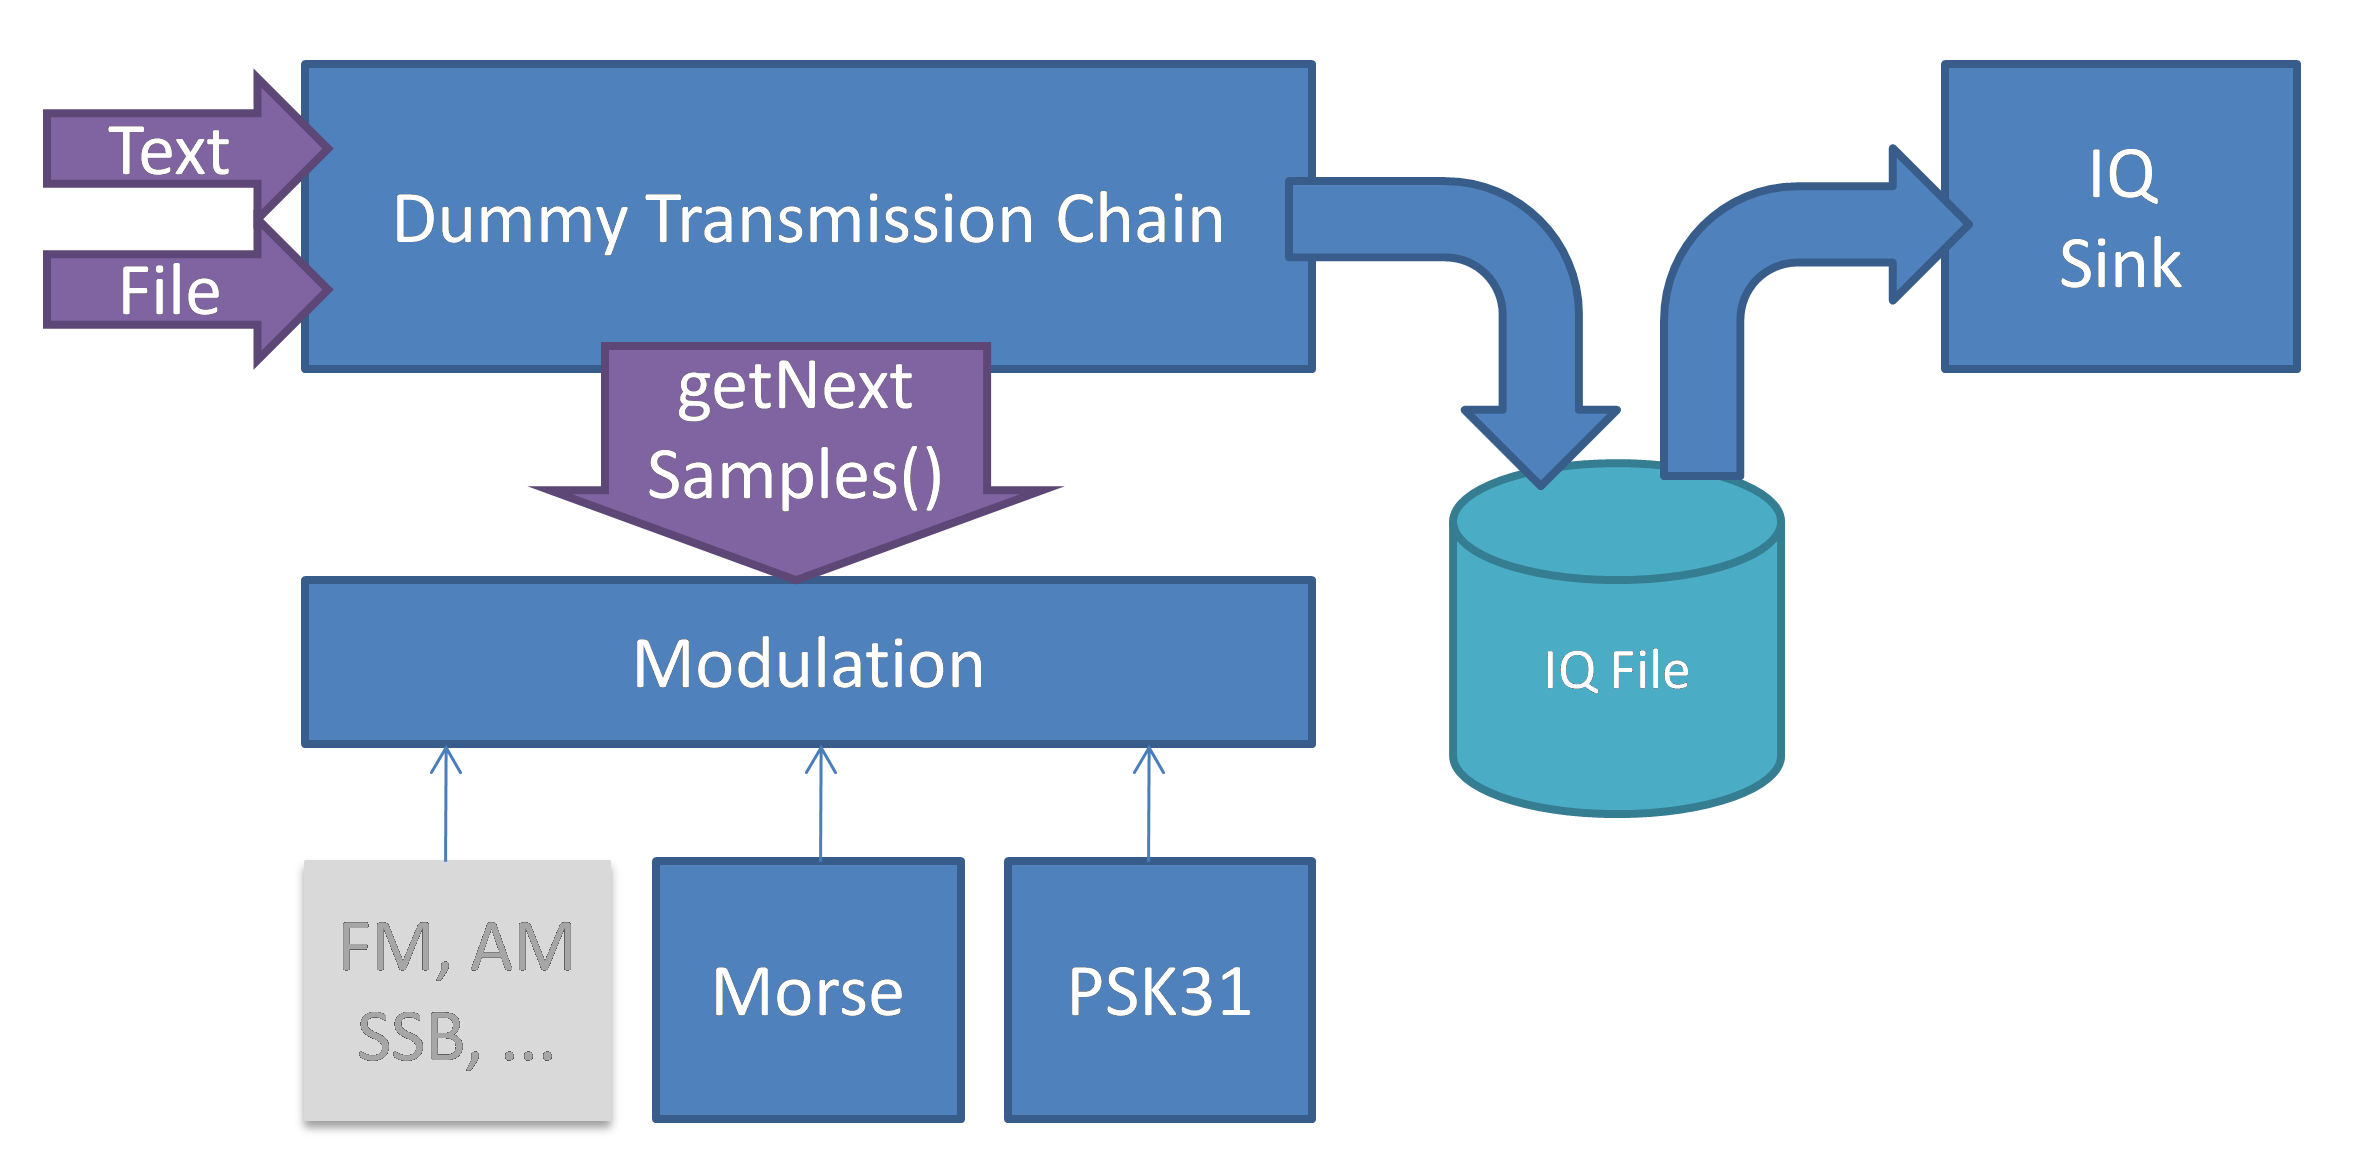
\includegraphics[width=1\linewidth]{gfx/TX_chain_step2.png}
	\caption{Transmission in current version of AnSiAn \cite{Mantz2016}}
	\label{fig:tx_chain_old}
\end{figure}

\begin{figure}
	\centering
	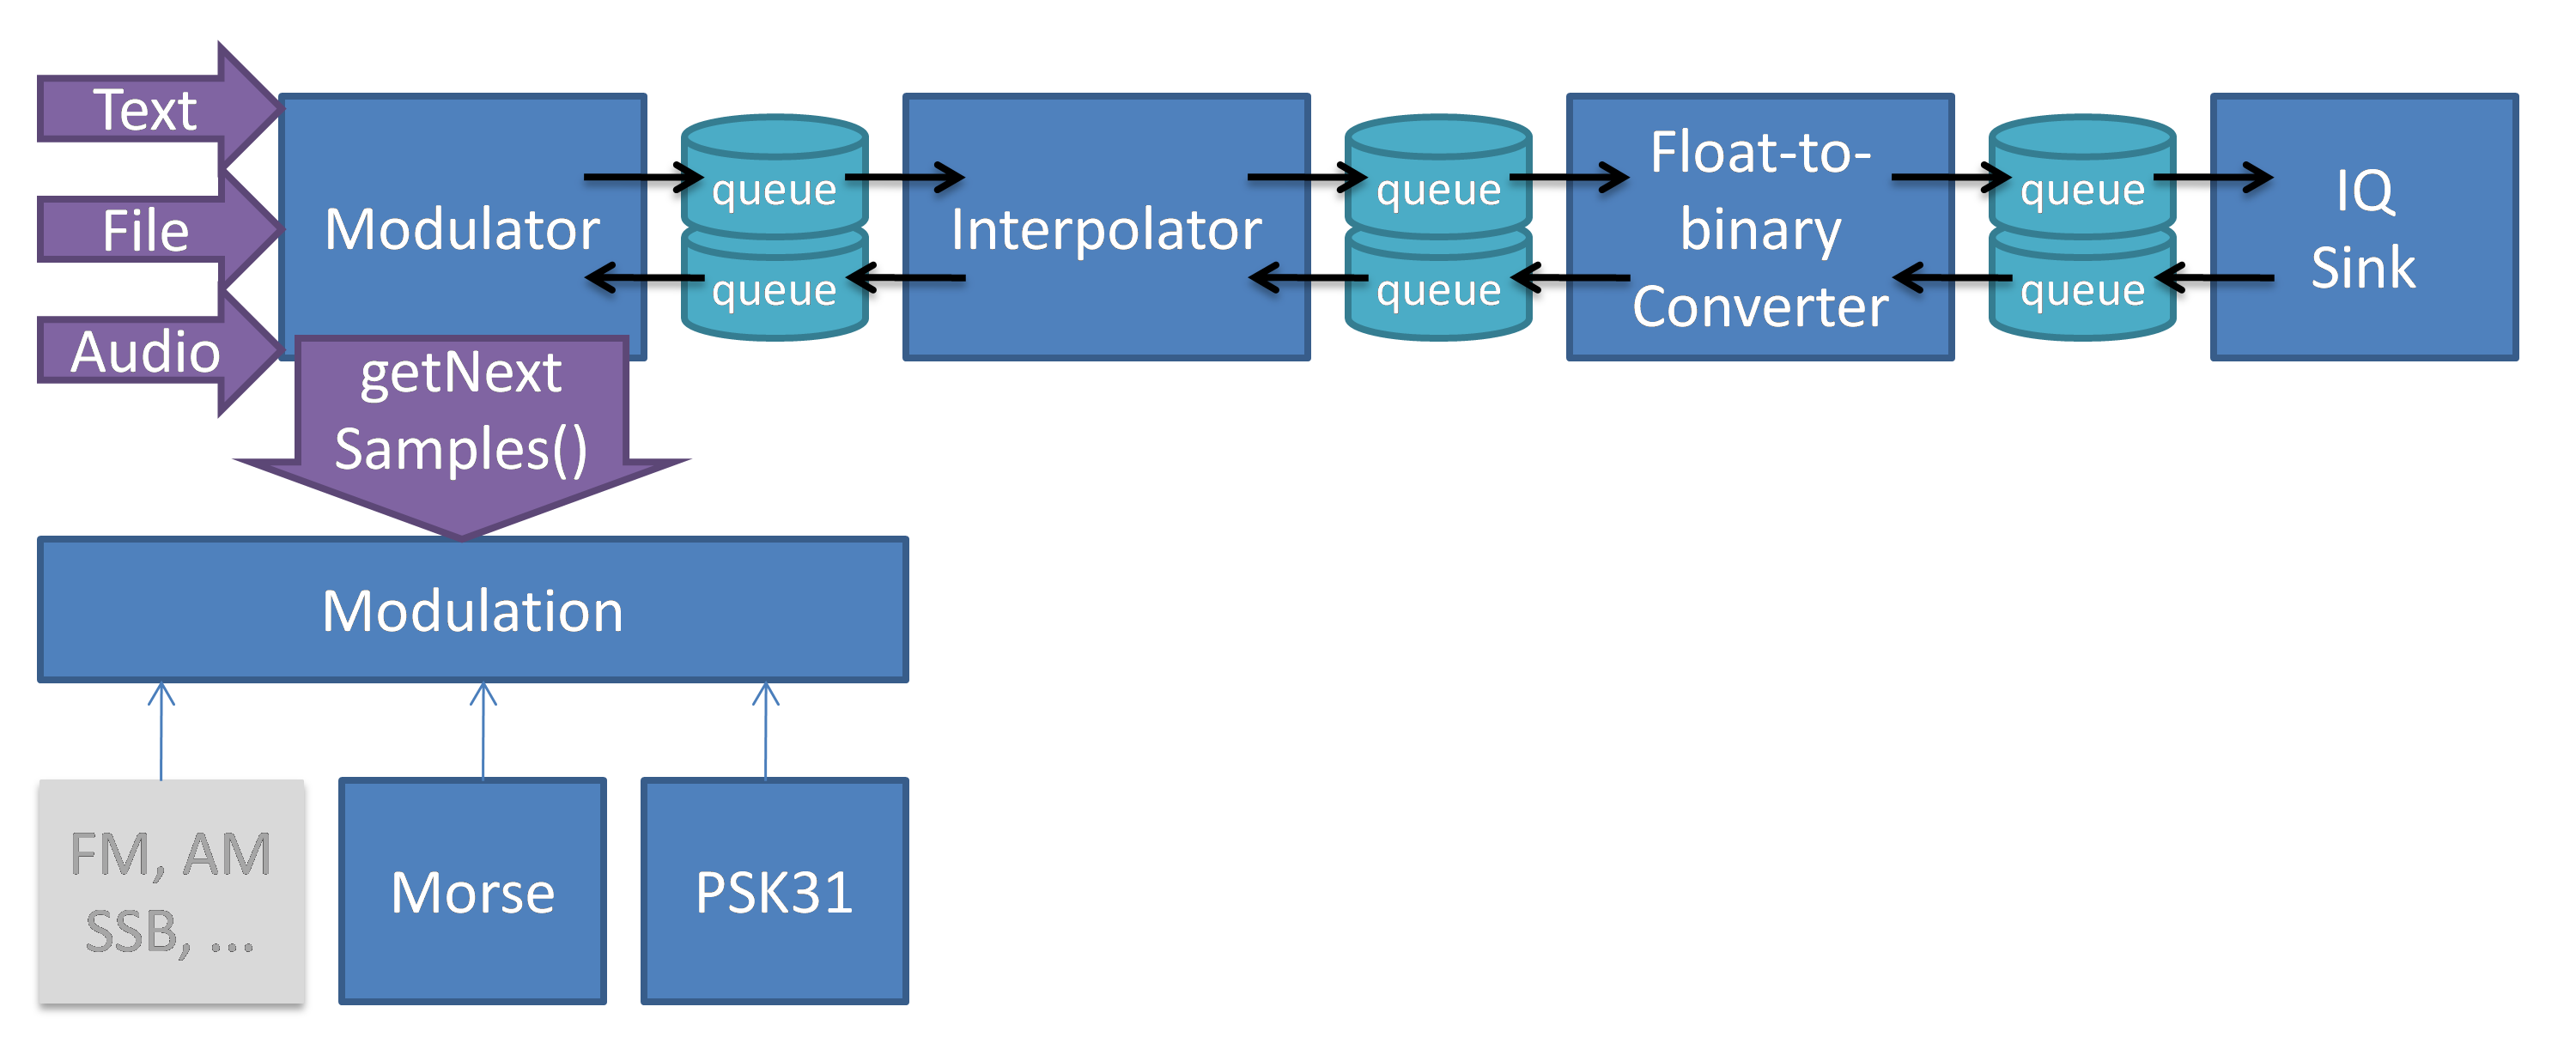
\includegraphics[width=1\linewidth]{gfx/TX_chain_final.png}
	\caption{Final transmission chain as suggested by \cite{Mantz2016}}
	\label{fig:tx_chain_new}
\end{figure}



\begin{figure}
	\centering
	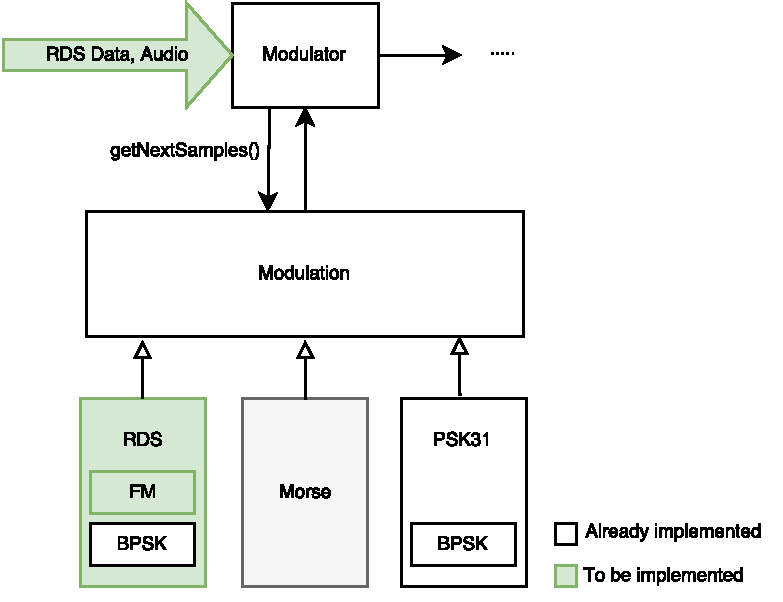
\includegraphics[width=1\linewidth]{gfx/feature2_components.pdf}
	\caption{Required Components for RDS Transmission}
	\label{fig:rds_transmission}
\end{figure}



\begin{figure}
	\centering
	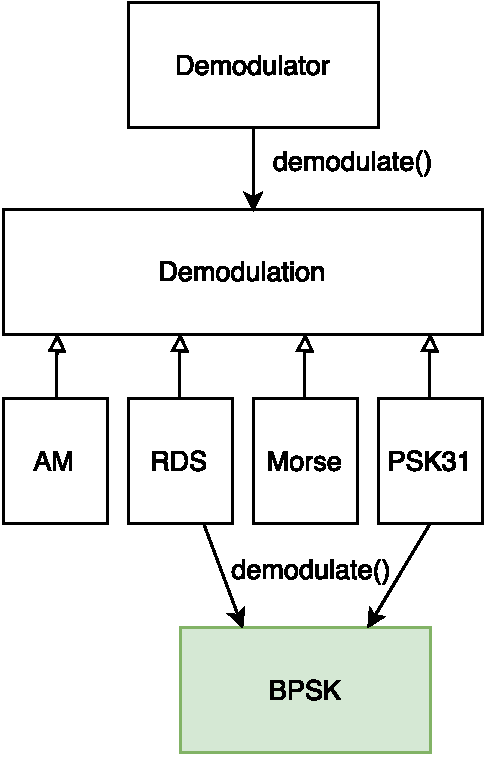
\includegraphics[width=0.5\linewidth]{gfx/feature3_components.pdf}
	\caption{Required Components for BPSK Demodulation Improvements}
	\label{fig:bpsk_components}
\end{figure}


\begin{figure}
	\centering
	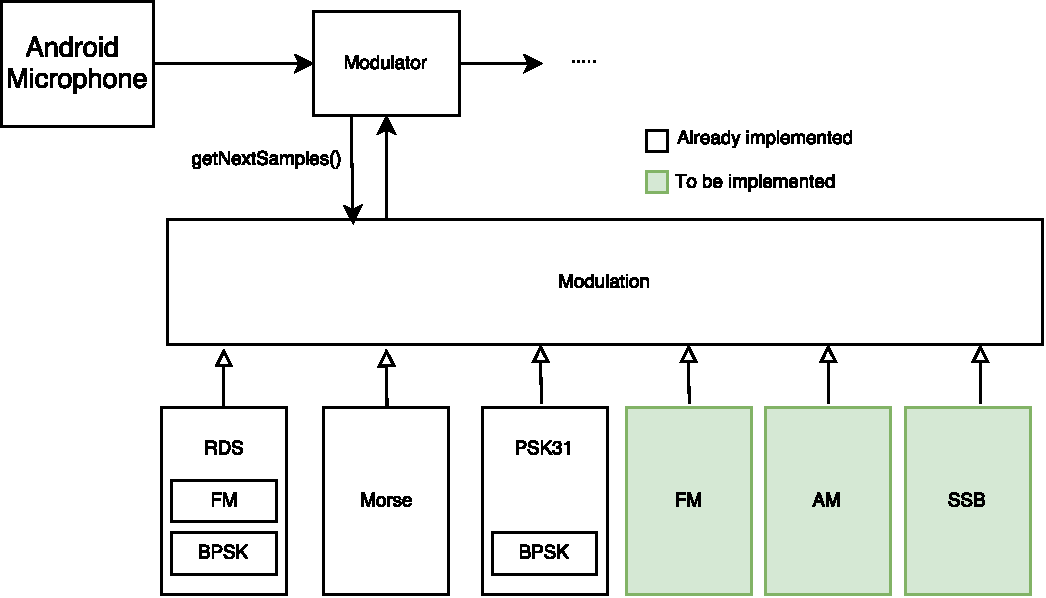
\includegraphics[width=1\linewidth]{gfx/feature4_components.pdf}
	\caption{Required Components for Walkie-Talkie-mode}
	\label{fig:walkie_talkie_components}
\end{figure}
% !TeX spellcheck = en_US

\chapter{Project Progress}

At the very beginning of this project a detailed project plan has been defined. We divided each feature into a list of subsequent tasks and estimated the work required to complete them. 

This chapter reviews the progress throughout the project. At the each release we analyze how much time has been spent on the single tasks and if our initial planning needs to be adapted.


\section{Alpha Release: 22.12.2016}

The goal was to implement feature 1 (Transmission Chain) and feature 2 (RDS Transmission). This goal has been achieved. Additionally we started to document the implementation, which was initially planned to be done at the end of the project. 

\begin{table}
\centering
\caption{Expected and Actual Workload for Features in Alpha Release}
\label{tab:alpha:features}
\begin{tabular}{ l | c | c }
	 & expected  & actual \\ \hline
	Transmission Chain & 50h & 24h \\  \hline
	RDS Transmission & 35h & 55h \\ \hline
	Documentation & 0h & 7h \\ \hline \hline
	Total & 85h & 86h 
\end{tabular}
\end{table}

Table~\ref{tab:alpha:features} shows the total workloads that were required to implement the features. We can see that we overestimated the transmission chain feature and underestimated the RDS feature. In total the required time is roughly as expected. 

\begin{table}
	\centering
	\caption{Expected and Actual Workload for Feature 1: Transmission Chain}
	\label{tab:alpha:feature1}
	\begin{tabular}{ l | c | c }
		& expected  & actual \\ \hline
		Task 1: Investigation of Existing Code & 5h & 3h \\  \hline
		Task 2: Rewrite Modulator  & 10h & 9h \\ \hline
		Task 3: Implementation Interpolator & 10h & 0h \\ \hline
		Task 4: Refactor Existing Code and Finalize & 5h& 2h  \\ \hline
		Task 5: Integration & 10h & 4h  \\ \hline
		Task 6: Regression Testing & 10h & 6h  \\ \hline \hline 
		Total & 50h & 24h 
	\end{tabular}
\end{table}

Table~\ref{tab:alpha:feature1} lists the single tasks for feature 1. We decided to leave out the interpolator at first (see Section~\ref{sec:impl:feature1}). All other tasks were much easier as expected. Even the integration and testing with the already existing transmission modes went very well. 
	
	\begin{table}
		\centering
		\caption{Expected and Actual Workload for Feature 2: RDS Transmission}				\label{tab:alpha:feature2}
		\begin{tabular}{ l | c | c }
			& expected  & actual \\ \hline
			Task 7: Investigation of Existing Code&  5h & 5h \\ \hline
			Task 8: Implementation in MATLAB & 5h & 6h  \\ \hline
			Task 9: Portation to Java & 15h & 17h  \\ \hline
			Task 10: Testing and Bug Fixing & 10h & 26h \\ \hline \hline
			Total & 35h & 55h
		\end{tabular}
	\end{table}
	
	Table~\ref{tab:alpha:feature2} evaluates the required time for the tasks in feature 2. Tasks 7, 8 and 9 were nearly completed within the expected time, while the testing and debugging took much longer than expected. We highly underestimated the complexity of finding bugs in signal processing code on Android. Since we are dependent on the HackRF hardware and driver, most of the testing needs to be done on the actual smartphone. This means that it requires a lot of manual work - although we tried to implement some automated testing (see \ref{sec:impl:feature2}). 
	
	\begin{figure}
		\centering
		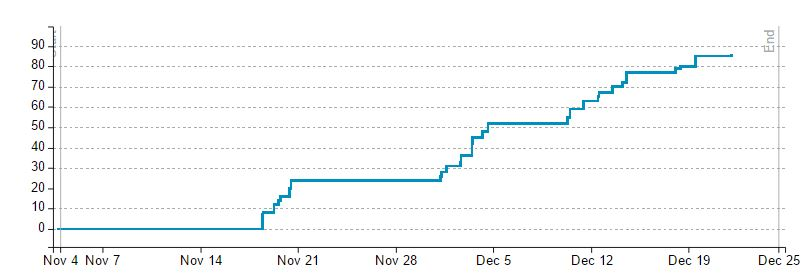
\includegraphics[width=1\linewidth]{gfx/Agilefant_Alpha.jpg}
		\caption{Workload Distribution for Alpha Release (04.11.2016-22.12.2016)}
		\label{fig:agilefant_alpha}
	\end{figure}
	
	Figure~\ref{fig:agilefant_alpha} gives the distribution of the workload as exported from our tracking tool Agilefant. The workload was not well distributed at the beginning, mainly focused on single weekends with long breaks in between. During the last weeks before the deadline this became slightly more distributed. 

\section{Beta Release: 02.02.2017}
The (ambitious) goal of this release was to finish all remaining features. This goal was not achieved, due to lack of time. However, we already finished a good portion of the documentation, which was initially planned for the final release. 

\begin{table}
	\centering
	\caption{Expected and Actual Workload for Features in Beta Release}
	\label{tab:beta:features}
	\begin{tabular}{ l | c | c }
		& expected  & actual \\ \hline
		Walkie Talkie & 60h & 65h \\  \hline
		BPSK Demodulation Improvement & 55h & 0h \\  \hline
		Documentation & 0h & 13h \\ \hline \hline
		Bug Fixing of previous features & 0h & 10h \\ \hline \hline 
		Total & 115h & 88h 
	\end{tabular}
\end{table}
Table~\ref{tab:beta:features} shows the expected and actual time spent implementing the features. The Walkie Talkie was expected to take 60 hours and was completed in 65 hours. The BPSK feature was expected to take 55 hours, but it was decided to exclude this feature, because the benefit of an improved BPSK demodulation implementation is not high enough. 
Additionally, we spent 13 hours creating this documentation and needed 10 unplanned hours to fix problems in the transmission chain and RDS implementation. In total we have spent 88 hours which is way below the planned value of 115 hours. 

In total we already spent 194 hours (20+86+88) on this project, such that we have 66 hours left. We are planning to use this time to implement \ac{SSTV}, to finalize the documentation and to prepare the final presentation. 


	\begin{table}
	\centering
	\caption{Expected and Actual Workload for Feature 4: Walkie Talkie}
	\label{tab:alpha:feature4}
	\begin{tabular}{ l | c | c }
		& expected  & actual \\ \hline
		Task 17: Design and Implement UI& 15h & 19h \\ \hline
		Task 18: Implementation AM& 15h & 0h  \\ \hline
		Task 19: Implementation FM& 10h & 18h  \\ \hline
		Task 20: Implementation SSB& 10h & 14h \\ \hline 
		Task 21: Testing and Bug Fixing& 10h & 14h \\ \hline \hline
		Total & 60h & 65h
	\end{tabular}
\end{table}

Table~\ref{tab:alpha:feature4} shows the actual time spent on each task in the Walkie Talkie feature. We underestimated every task. The implementation of AM was excluded, because it is not widely used. 
Figure~\ref{fig:agilefant_beta} shows the distribution of the workload over the time for the beta release. We see that there was no activity during the last week of December and first week of January (other than planned). The weeks after that are roughly evenly distributed. 

\begin{figure}
	\centering
	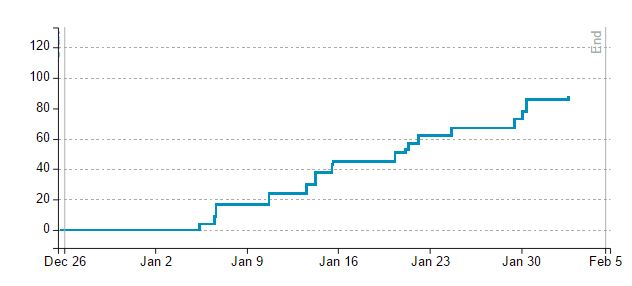
\includegraphics[width=1\linewidth]{gfx/Agilefant_Beta.jpg}
	\caption{Workload Distribution for Beta Release (23.12.2016-02.02.2017)}
	\label{fig:agilefant_beta}
\end{figure}

\section{Final Release: 09.03.2017}

\begin{table}
	\centering
	\caption{Expected and Actual Workload for Features in final Release}
	\label{tab:final:features}
	\begin{tabular}{ l | c | c }
		& expected  & actual \\ \hline
		SSTV & 50h & 58h+ \\  \hline
		Documentation & 25h & 21h \\ \hline \hline
		Presentation & 15h & 15h \\ \hline \hline 
		Total & 90h & 94h  
	\end{tabular}
\end{table}


In this final release, we completed the documentation and prepared the final presentation. Other than initially planned, we decided after the beta release to implement \ac{SSTV} instead of improving \ac{BPSK} and implementing \ac{QAM}. Therefore, the expected workloads for those features became irrelevant. We estimated that we would be able to implement the SSTV feature in 50 hours. Table~\ref{tab:final:features} shows the actual workload for this release. We see that we spent 58 hours on the SSTV feature and there are still parts that are currently not working properly. The documentation and presentation have been completed in the expected time, but other than initially planned we spent a good amount on the documentation in the previous releases. Therefore, the total documentation time is higher than expected. 

\begin{figure}
	\centering
	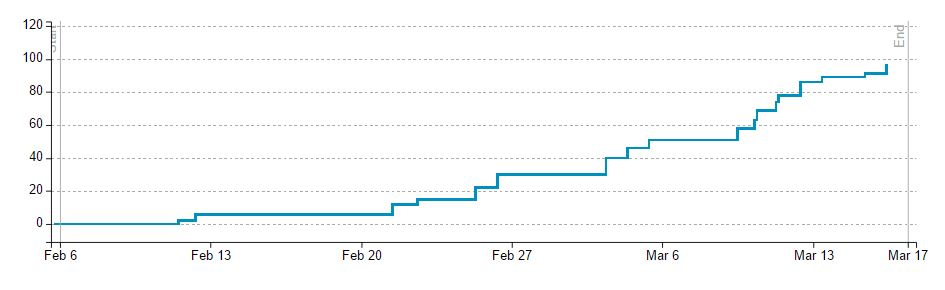
\includegraphics[width=1\linewidth]{gfx/Agilefant_Final.jpg}
	\caption{Workload Distribution for Final Release (03.02.2017-17.03.2017)}
	\label{fig:agilefant_final}
\end{figure}

Figure~\ref{fig:agilefant_final} shows the distribution of the work load over the time frame. The majority of the work was done in the last 3 weeks, due to other exams and vacation. 


\chapter{Implementation}

This chapter describes the implementation of the features that were added to \ac{AnSiAn}. We roughly describe the theoretical background, the design choices made and the actual implementation in Java. Additionally we extensively describe the challenges we faced during the implementation. 

\section{Feature 1: Transmission Chain}


\begin{figure}
	\centering
	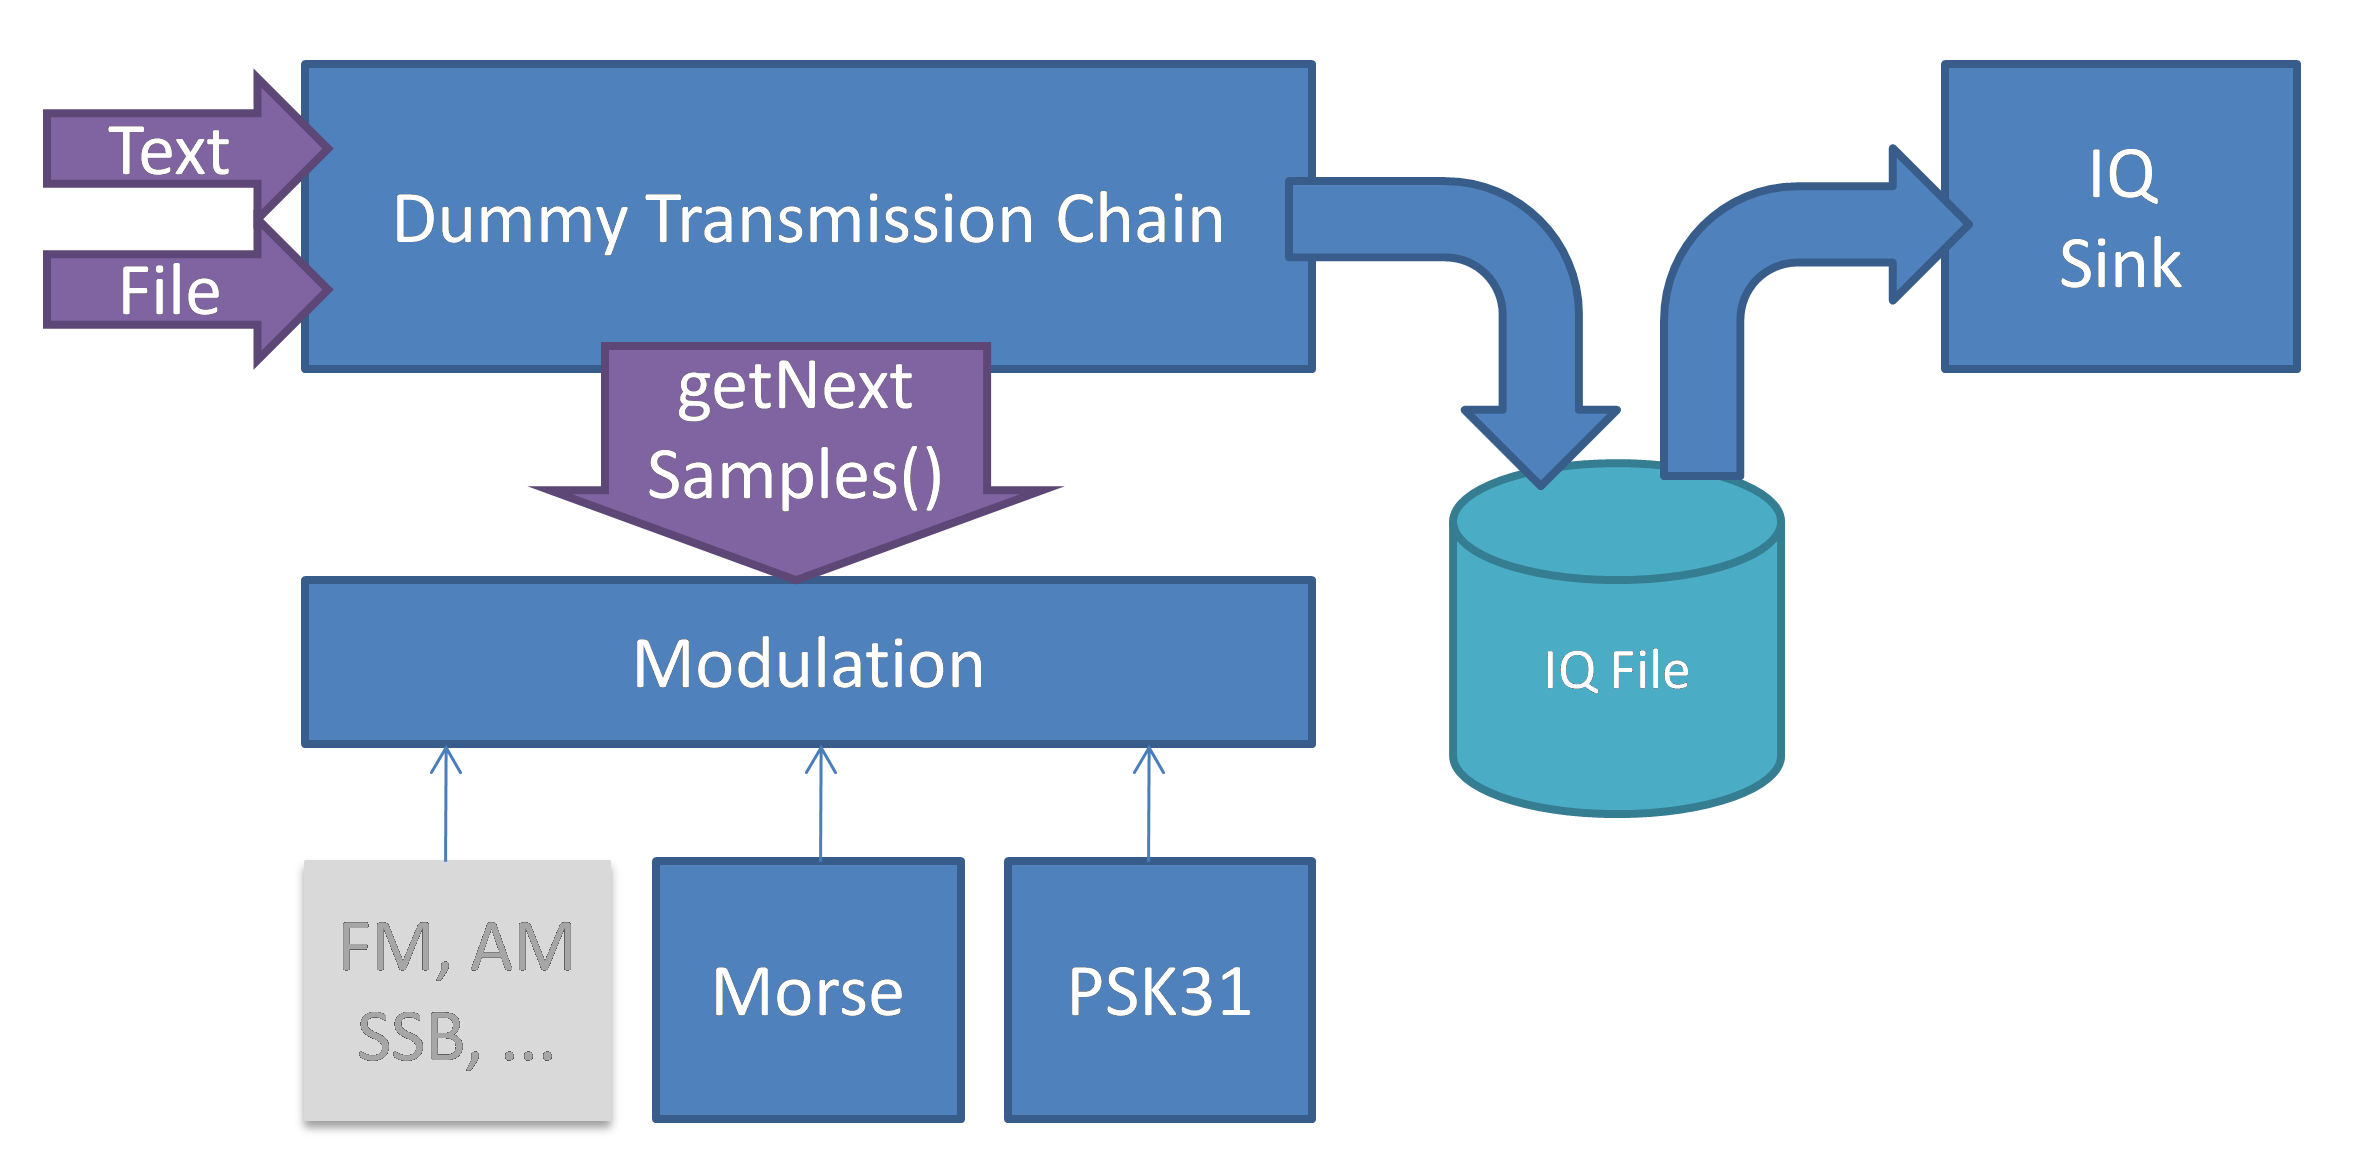
\includegraphics[width=1\linewidth]{gfx/TX_chain_step2.png}
	\caption{Transmission in current version of AnSiAn \cite{Mantz2016}}
	\label{fig:tx_chain_old2}
\end{figure}


Figure~\ref{fig:tx_chain_old2} illustrates the implementation of the transmission before our project started. We roughly analyze how this has been implemented to find out the main problems of the implementation. The DummyTransmissionChain is the entry point of a transmission. It is called when the user initializes a transmission. The different modulations (currently PSK31 and Morse) are implemented as a subclass of Modulation. The DummyTransmissionChain repeatedly calls getNextSamples() to get a SamplePacket of the selected Modulation until it returns null. The SamplePacket is basically a complex array (i.e. 2 float arrays containing in-phase and quadrature components). The DummyTransmissionChain then serializes this to a signed 8 bit integer IQ File, i.e. converts floats to bytes and interleaves I and Q samples. Once the Modulation is done, the IQSink is launched which reads the file and passes it to the HackRF driver using the BlockingQueue of byte buffers provided by the HackRF driver. 

\pagebreak
With this implementation we see the following problems: 
\begin{itemize}
	\item The modulation is entirely done before the transmission is start-ed. This is not only very inconvenient for the user since he has to wait for a long time before the transmission starts, but it also is not suitable for the features we want to implement where we require continuous transmission of recorded audio. We want to implement this in a way where the modulation is done simultaneously to the transmission. Mantz and Engelhardt \cite{Mantz2016} already described a concept to use BlockingQueues, i.e. we queue up N packets and then block until a packet has been removed from the queue. This helps to have enough samples ready, but not using too much memory, which is a rare resource on smartphones. 
	\item Writing to a file introduces additional overhead. This was done to save memory, but is not required if we can do the modulation just-in-time. 
	\item The format of the file is currently limited to interleaved I/Q 8-bit signed integers. It would be nice to support other formats as well. 
	\item Aborting a transmission currently takes a few seconds due to the implementation of the IQ Sink. 
	\item Currently only the sampling rate of 1MHz is supported. This is not a real problem at the moment, but it might be nice in the future to be able to use different input and output sample rates for the transmission chain.
\end{itemize}

\label{sec:impl:feature1}
\subsection{Structural Changes}
\begin{figure}
	\centering
	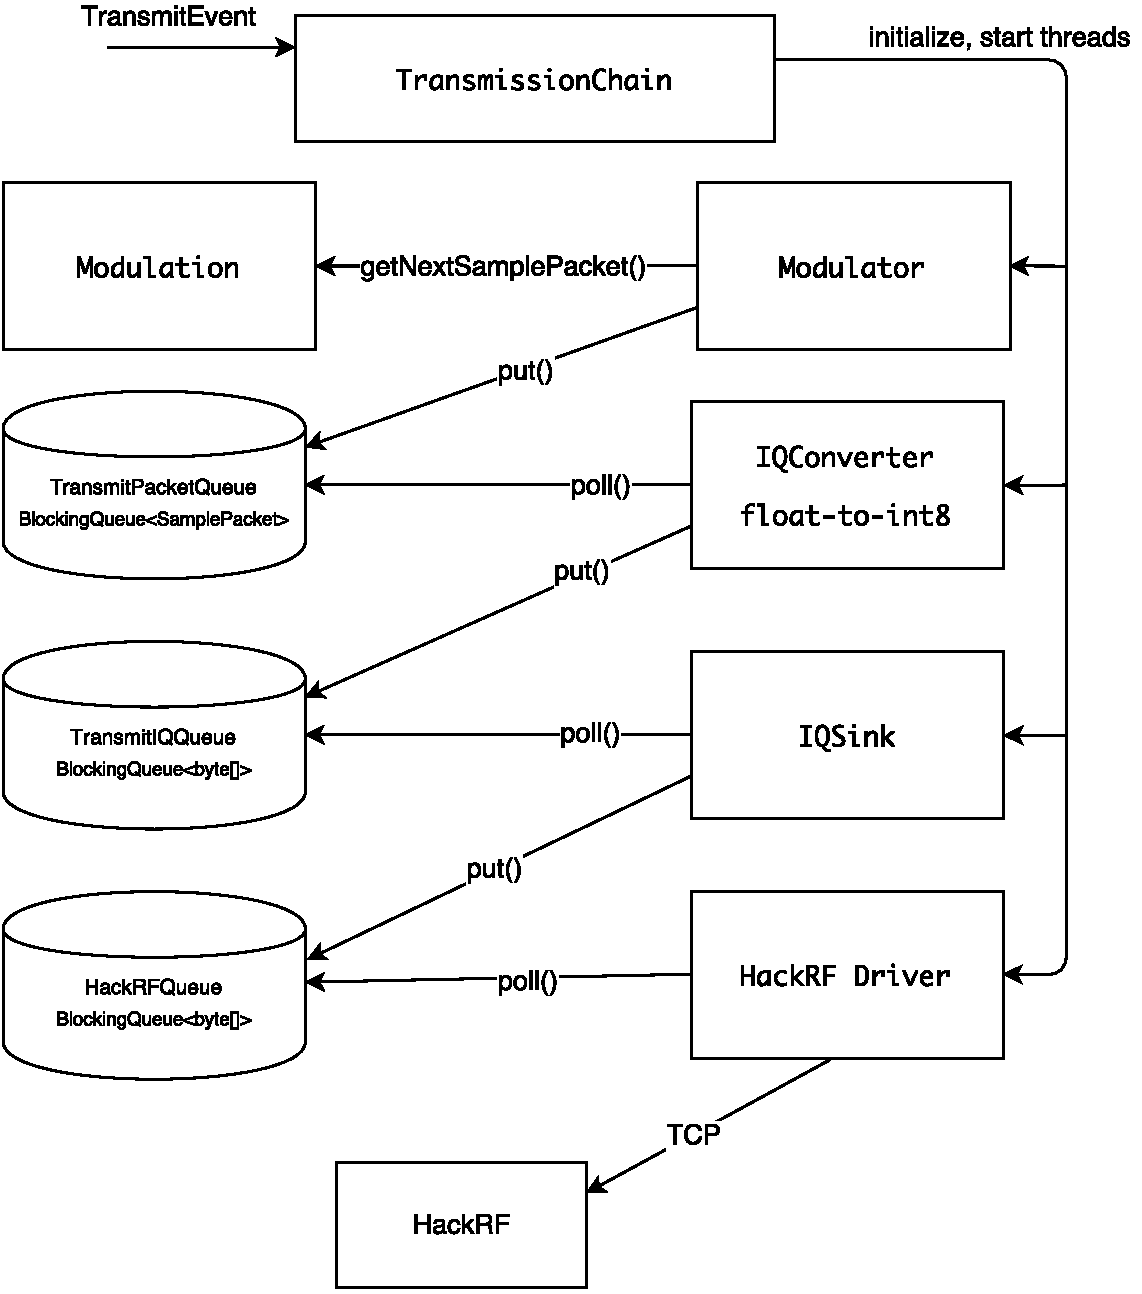
\includegraphics[width=0.8\linewidth]{gfx/feature1_design.pdf}
	\caption{Implementation of the Transmission Chain}
	\label{fig:impl:transmissionchain}
\end{figure}
To solve the problems detected with the old implementation we needed to adjust the architecture of the transmission chain. The current transmission chain is outlined in Figure~\ref{fig:impl:transmissionchain}. We briefly describe the responsibilities of each component: 

\begin{itemize}
	\item \textbf{TransmissionChain}: Responsible to launch the transmission chain. It listens to TransmitEvents that were sent by the UI. It is the only object that is created on app startup and is kept in memory for the entire time - all other parts of the transmission chain are started for a single transmission and die afterwards. Ideally this class is the only one that contains Android specific / dependent code. 
	\item \textbf{Modulator}: The Modulator continuously gets SamplePackets from the correct Modulation and pushes them to the TransmitPacketQueue. 
	\item \textbf{IQConverter}: Converts the SamplePackets (float) from the TransmitPacketQueue to the required data format (For HackRF: 8bit IQ samples). The data is filled into byte buffers that are then enqueued into the TransmitIQQueue. 
	\item \textbf{IQSink}: Configures the HackRF Driver. Then continuously takes the buffers from the TransmitIQQueue and passes them to the driver specific Queue. 
\end{itemize}

We decided not to implement an interpolator at first, which would have enabled to use different sampling rates for modulating than for the actual transmission. We did this because currently we are using 1 MHz everywhere. If we require different sampling rates later this can be easily added. 

\subsection{Implementation}

After we described the structural changes and required classes in the last section, we now point out a few specific implementation choices that were made during the development: 
Since we need to run the components concurrently and we do not want to do a lot of work on the main thread, we need to make use of multiple threads. When a transmission is initialized the TransmissionChain object quickly creates a object of each component and then runs each in a separate thread. \\
We already described the concept of Blocking Queues. This highly simplifies the implementation of the chain, since we do not need to take of the communication and memory management. The threads just do their work and enqueue the results in the next queue and the rest is controlled by the queue limits. We only need to decide how long the queues are. The byte buffers have a size of 16 KiB (as defined by the HackRF driver), while the SamplePackets can have arbitrary size (usually a lot bigger). Therefore we currently choose 5 as the maximum size of the TransmitPacketQueue and 200 for the TransmitIQQueue.  
	
It is important to keep memory management in mind. If every component just keeps allocating new memory the application will run out of memory or the Java Garbage Collector will be to busy and drastically slow down the application. Therefore we use the buffer pool for the byte buffers of the HackRF driver. This again uses BlockingQueues, which makes sure that only a fixed number of buffers are used throughout the application.  
	
All components need to be interruptible. This needs to be implemented by the class itself. The TransmissionChain can only call the .interupt method of the thread, but the thread itself needs to take care that this interupt is received and correctly handled. 
	
The implementation of the IQConverter was more challenging than expected. The main challenge is that the size of the SamplePackets can be different than and even not divisible by the buffer size required by the IQSink. We decided to memorize the last samples of the SamplePacket until the next SamplePacket is processed. However we can not know if a SamplePacket is the last one. Therefore we implemented that that if no SamplePacket arrives for a specified time (here 1000 ms), we fill the rest of the buffer with zeros and transmit it. 


\subsubsection{Debugging and Testing}
Since all software contains bugs, we needed to find a way to find a way to debug and test our implementation in a convenient and fast way. We developed unit tests for the IQConverter, since it contains logic that can be easily tested by a unit test. 

To test the other components we wanted to monitor the bytes that are actually passed to the HackRF driver. To do so we implemented a FileIQSink, that can be launched instead of the normal IQSink. This FileIQSink writes the samples to a file. Then we transfered this file to a computer and analyzed them with Matlab, Audacity and a Hex editor. 
After we successfully fixed a lot of smaller bugs in our implementation, we integrated it into the current application and performed manual regression tests of the already implemented transmission features. We tested our implementation with the 3 currently implemented transmission modes: 
\begin{itemize}
	\item Morse Code Modulation
	\item PSK31 with USB Modulation
	\item Directly transmitting a IQ File 
\end{itemize}

All three transmission modes are now working without any problems and do no longer require long calculations before the transmission. 



\section{Feature 2: RDS Transmission}
\label{sec:impl:feature2}
The second feature implements the synthesis of \ac{RDS} signals. \ac{RDS} has been standardized by the RDS Forum \cite{RDS1999}. It is a good example for a non-trivial protocol that is very widely used. We wanted to demonstrate that these signals can be synthesized on a smartphone, such that a commodity kitchen or car radio is able to decode them. 

One of the main features of RDS is the transmission of the station information (station name, audio information, station location and other meta data about the transmission). Most radios only display the station name. This is why we are also concentrating on this feature. 

The RDS signals are transmitted together with the audio signal using frequency modulation. By implementing RDS in AnSiAn, we enables the user to broadcast his own radio signals with a station name specified by the user. 

\subsection{User Interface}
\begin{figure}
	\centering
	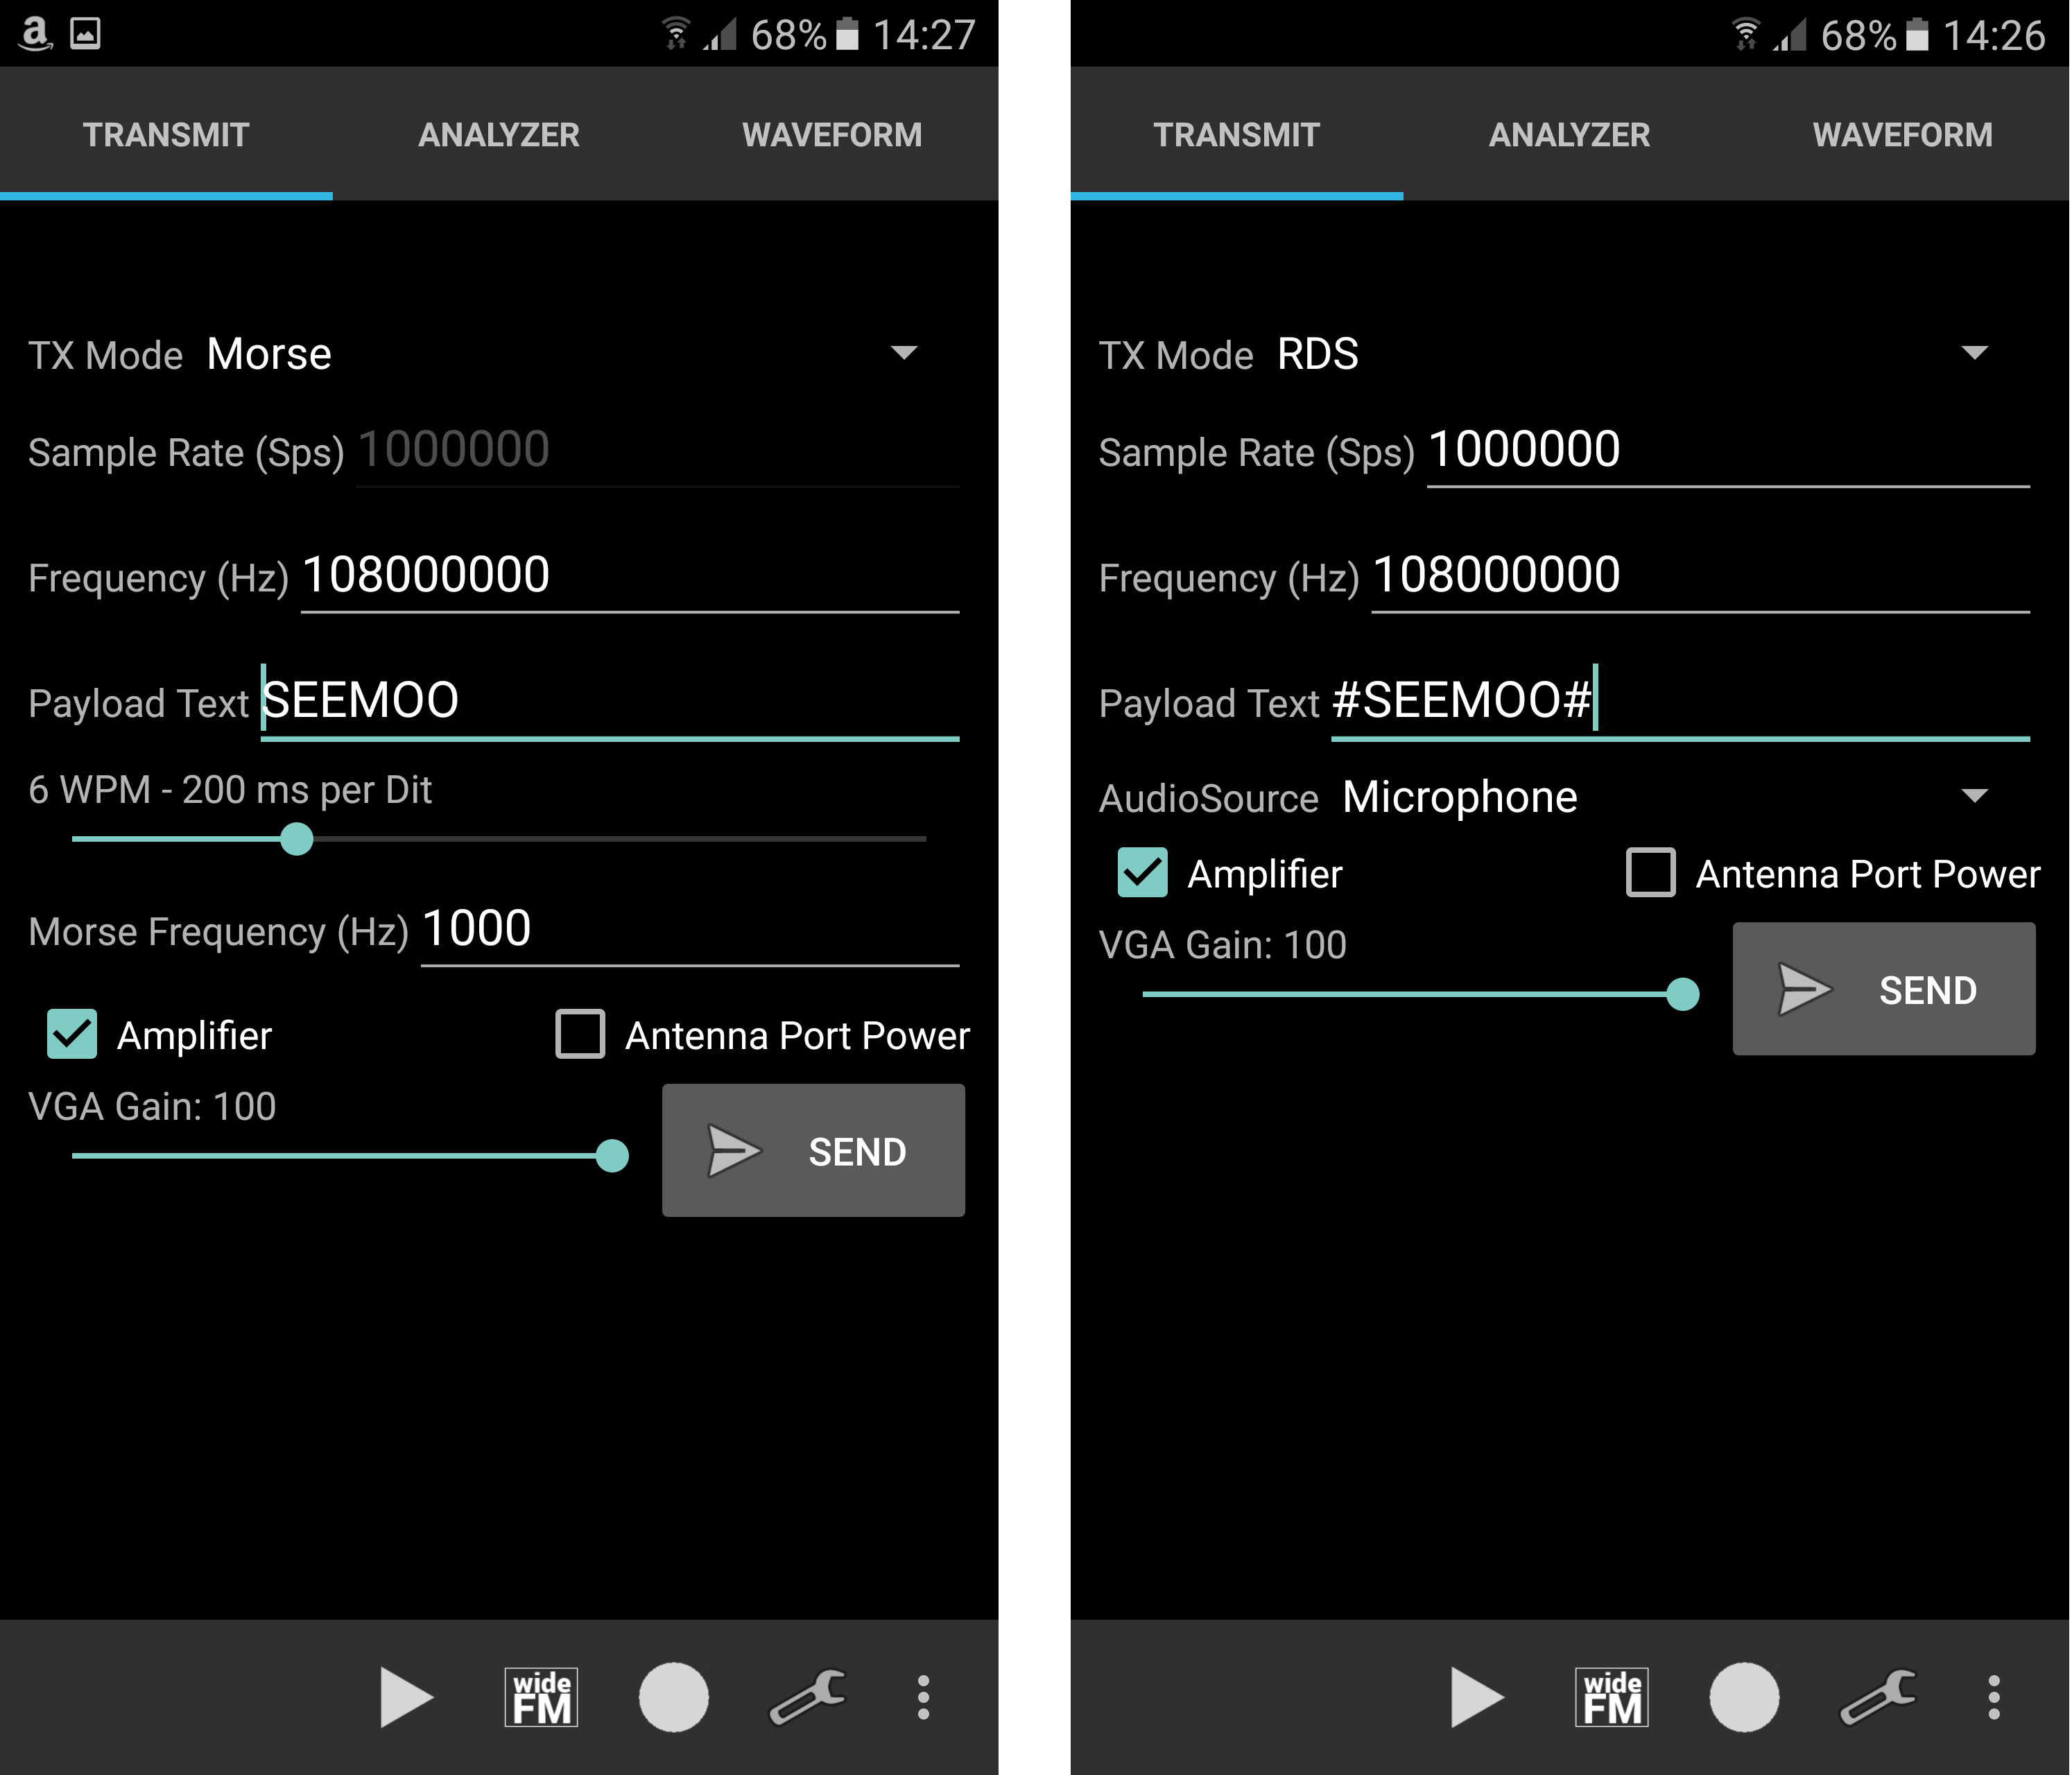
\includegraphics[width=1.0\linewidth]{gfx/screenshot_rds.png}
	\caption{AnSiAn Transmission Tab: Morse (old, left) and RDS (new, right)}
	\label{fig:impl:screenshotrds}
\end{figure}


Figure~\ref{fig:impl:screenshotrds} shows a screenshot of the extended transmission tab of AnSiAn. For reference we printed the already existing Morse transmission screen on the left. On the right you can see the newly added screen which enables the user to transmit RDS signals. The user can enter his own station name (at most 8 characters) and select an audio source (currently we are supporting the integrated microphone and a audio file source). The other settings are the same as for the other transmission modes. 


\subsection{Implementation}
To transmit a radio signal including RDS, we need to do the following steps (c.f. \cite{RDS1999}):

\begin{enumerate}
	\item Generate a bit string according to RDS specification (4 groups, each 64 bit)
	\item Calculate 10 bit check words for every 16-bit block (resulting in 4 groups, each 104 bits)
	\item Calculate differential encoding of the bit string
	\item Manchester encode the bit string
	\item Apply a low-pass filter to the signal to cut off frequencies higher than 2800 Hz
	\item Upconvert the generated signal to 57 kHz
	\item Add a sinusoidal pilot tone at 19 kHz
	\item Add the base band audio signal (only containing low frequencies). Most audio signals are sampled at 44100 Hz. So we need to resample these signals to match our sampling rate of 1MHz. 
	\item Calculate the frequency modulation on the signal with a frequency deviation of 75000 kHz 	
\end{enumerate}

\begin{figure}
	\centering
	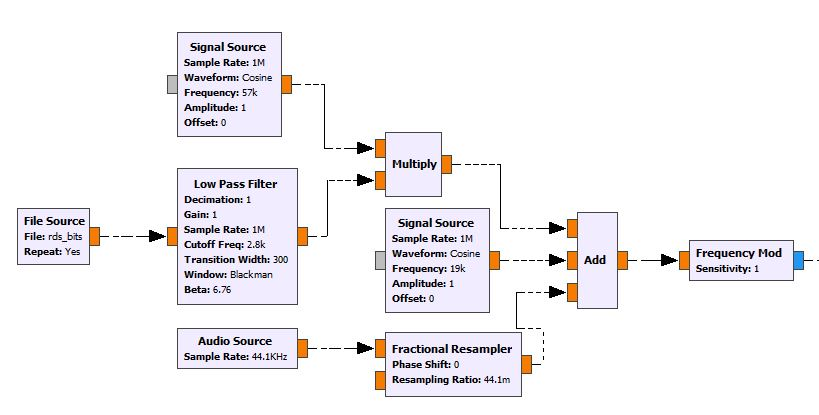
\includegraphics[width=1.3\linewidth]{gfx/rds_gnu.jpg}
	\caption{GNU Radio flow graph of RDS signal generation}
	\label{fig:impl:rdsgnu}
\end{figure}

The steps after step 4 are illustrated in the GNU radio flow graph in Figure~\ref{fig:impl:rdsgnu}. Since most of these steps are pretty straight forward we only explain the more complex ones in detail here. For the bit string generation and check word calculation refer to the documentation of the RDS decoding functionality implemented in AnSiAn (The documentation of that can be found in \cite{Mantz2016} in Section 4.2.3). 

\subsubsection{Low-Pass Filtering}

AnSiAn already contains a implementation of a Blackman Low-Pass filter. The signature of the low pass filter function is shown in Listing~\ref{lst:javacreatelowpass}

\begin{lstlisting}[label=lst:javacreatelowpass, caption=AnSiAn Blackman Low-Pass Filter, language=java]
// create a filter 
public static FirFilter createLowPass(int decimation, float gain, 
   float sampling_freq, // Hz
   float cutoff_freq, // Hz BEGINNING of transition band
   float transition_width, // Hz width of transition band
   float attenuation_dB) // attenuation dB
   
// filter 
public int filterReal(SamplePacket in, SamplePacket out, int offset, int length)    

\end{lstlisting}
However the choice of its parameter highly influences the performance of the filter. A bad parameter choice either leads to a badly filtered signal or to a very long filtering time. Since we are very constrained in terms of computing power on the Android platform, we want to choose the parameter such that the filter is just good enough but still very fast. 
We found that the best parameter choice for us was cutoff\_freq=2800Hz, transition\_width=300Hz and attenuation\_dB=3dB. \\
The parameters decimation=1, gain=1 and sampling\_freq=1000000 are fixed for us. 

\subsubsection{Frequency Modulation}

For implementing frequency modulation, we looked the implementation in the Octave communications package. Listing~\ref{lst:octave_fmmod} shows how Octave implements fmmod. 
\lstset{numbers=left}
\lstset{stepnumber=1}
\begin{lstlisting}[label=lst:octave_fmmod, caption=Octave implementation of Frequency modulation \cite{octavefmmod}, language=octave,]
function s = fmmod (m, fc, fs, freqdev)
   l = length (m);
   t = 0:1./fs:(l-1)./fs;
   int_m = cumsum (m)./fs;
   s = cos (2*pi.*fc.*t + 2*pi.*freqdev.*int_m);
endfunction
\end{lstlisting}

It implements the following function 

\begin{equation}
 s(t) = cos\left(2\cdot \pi \cdot f_c \cdot t + 2\cdot \pi\cdot f_\Delta \int_{0}^{t}m(t')dt'\right)
\end{equation}

However this modulates the signal in the pass band, but we require it in the base band and the up conversion is done later by the HackRF. Therefore we can either set $f_c=0$ or use 

\begin{equation}
s(t) = cos\left(2\cdot \pi \cdot f_\Delta  \cdot \int_{0}^{t}m(t')dt'\right)
\end{equation}


The implementation in Java is straight forward and shown in Listing~\ref{lst:javafmmod}.
\begin{lstlisting}[label=lst:javafmmod, caption=Java Implementation of fmmod, language=java,]
public static SamplePacket fmmod(float[] x, float fs, float freqdev ){
   SamplePacket packet = new SamplePacket(x.length);
   packet.setSize(x.length);
   float[] sum = cumsum(x);
   for(int i=0;i<sum.length;i++){
      sum[i] = sum[i]/fs;
   }
	
   float[] re = packet.getRe();
   float[] im = packet.getIm();
   for(int i=0;i<sum.length;i++){
      re[i] = (float) Math.cos(2*Math.PI*freqdev*sum[i]);
      im[i] = (float) Math.sin(2*Math.PI*freqdev*sum[i]);
   }
   return packet;
}

\end{lstlisting}



\subsection{Testing} 
Testing a transmission implementation can be very tedious, since even small bugs lead to a non-decodable signal. Therefore we again used the FileSink to write the generated signals to a file instead of transmitting them with the HackRF. We analyzed these signals and compared the intermediate results to a reference implementation of RDS in Matlab. 

Now AnSiAn is able to send RDS signals which can be decoded by commodity radios like the car radio in Figure~\ref{fig:impl:picrds}.

\begin{figure}
	\centering
	\includegraphics[width=1.0\linewidth]{gfx/feature2_pic.jpg}
	\caption{Decoded RDS signal on car radio}
	\label{fig:impl:picrds}
\end{figure}

\subsection{Performance issues}

TODO: describe performance issues, describe improvements , compare performance before and after 


% ********************************************************************
% Backmatter
%*******************************************************
\appendix
\cleardoublepage
%\ctparttext{The appendix contains some additional developments, that strongly supported us in the design of our communication system. Furthermore, it contains solutions to some problems.}
%\part{Appendix}
%\include{Parts/Part04}
%\include{Chapters/Part04_Chapter04_OOWARPLab}
%********************************************************************
% Other Stuff in the Back
%*******************************************************
\cleardoublepage%********************************************************************
% Bibliography
%*******************************************************
% work-around to have small caps also here in the headline
\manualmark
\markboth{\spacedlowsmallcaps{\bibname}}{\spacedlowsmallcaps{\bibname}} % work-around to have small caps also
%\phantomsection 
\refstepcounter{dummy}
\addtocontents{toc}{\protect\vspace{\beforebibskip}} % to have the bib a bit from the rest in the toc
\addcontentsline{toc}{chapter}{\tocEntry{\bibname}}
\label{app:bibliography}
\printbibliography
%\bibliography{Bibliography}
%\cleardoublepage\pagestyle{empty}

\hfill

\vfill


\pdfbookmark[0]{Colophon}{colophon}
\section*{Colophon}
This document was typeset using the typographical look-and-feel \texttt{classicthesis} developed by Andr\'e Miede. 
The style was inspired by Robert Bringhurst's seminal book on typography ``\emph{The Elements of Typographic Style}''. 
\texttt{classicthesis} is available for both \LaTeX\ and \mLyX: 
\begin{center}
\url{http://code.google.com/p/classicthesis/}
\end{center}
Happy users of \texttt{classicthesis} usually send a real postcard to the author, a collection of postcards received so far is featured here: 
\begin{center}
\url{http://postcards.miede.de/}
\end{center}
 
\bigskip

\noindent\finalVersionString

%Hermann Zapf's \emph{Palatino} and \emph{Euler} type faces (Type~1 PostScript fonts \emph{URW
%Palladio L} and \emph{FPL}) are used. The ``typewriter'' text is typeset in \emph{Bera Mono}, 
%originally developed by Bitstream, Inc. as ``Bitstream Vera''. (Type~1 PostScript fonts were made 
%available by Malte Rosenau and
%Ulrich Dirr.)

%\paragraph{note:} The custom size of the textblock was calculated
%using the directions given by Mr. Bringhurst (pages 26--29 and
%175/176). 10~pt Palatino needs  133.21~pt for the string
%``abcdefghijklmnopqrstuvwxyz''. This yields a good line length between
%24--26~pc (288--312~pt). Using a ``\emph{double square textblock}''
%with a 1:2 ratio this results in a textblock of 312:624~pt (which
%includes the headline in this design). A good alternative would be the
%``\emph{golden section textblock}'' with a ratio of 1:1.62, here
%312:505.44~pt. For comparison, \texttt{DIV9} of the \texttt{typearea}
%package results in a line length of 389~pt (32.4~pc), which is by far
%too long. However, this information will only be of interest for
%hardcore pseudo-typographers like me.%
%
%To make your own calculations, use the following commands and look up
%the corresponding lengths in the book:
%\begin{verbatim}
%    \settowidth{\abcd}{abcdefghijklmnopqrstuvwxyz}
%    \the\abcd\ % prints the value of the length
%\end{verbatim}
%Please see the file \texttt{classicthesis.sty} for some precalculated 
%values for Palatino and Minion.
%
%    \settowidth{\abcd}{abcdefghijklmnopqrstuvwxyz}
%    \the\abcd\ % prints the value of the length





\cleardoublepage% ******************************************************* Declaration
% *******************************************************
\refstepcounter{dummy}
%\pdfbookmark[0]{Thesis Statement}{statement} \chapter*{Thesis Statement}
\thispagestyle{empty}
\begingroup
%\let\cleardoublepage\relax
%\begin{flushright}
%	\emph{pursuant to §\,22 paragraph 7 of APB TU Darmstadt}
%\end{flushright}
%I herewith formally declare that I have written the submitted \myDegree{} independently. I did not use any outside support except for the quoted literature and other sources mentioned in the paper. I clearly marked and separately listed all of the literature and all of the other sources which I employed when producing this academic work, either literally or in content. This thesis has not been handed in or published before in the same or similar form.
%In the submitted thesis the written copies and the electronic version are identical in content.

%\bigskip

%\noindent\textit{\myLocation, \myTime}

%\smallskip

%\begin{flushright}
%	\begin{tabular}{m{5cm}}
%		\\ \hline
%		\centering\myName \\
%	\end{tabular}
%\end{flushright}

%\vfill

\selectlanguage{ngerman}
\pdfbookmark[0]{Erklärung}{erklaerung} \chapter*{Erklärung}
\begin{flushright}
	\emph{gemäß §\,22 Abs.\,7 APB der TU Darmstadt}
\end{flushright}
Hiermit versichere ich die vorliegende \myDegree{} ohne Hilfe Dritter und nur mit den angegebenen Quellen und Hilfsmitteln angefertigt zu haben. Alle Stellen, die Quellen entnommen wurden, sind als solche kenntlich gemacht worden. Diese Arbeit hat in gleicher oder ähnlicher Form noch keiner Prüfungsbehörde vorgelegen.
In der abgegebenen Arbeit stimmen die schriftliche und elektronische Fassung überein.

\bigskip
 
\noindent\textit{\myLocation, \myTime}

\smallskip

\begin{flushright}
    \begin{tabular}{m{5cm}}
        \\ \hline
        \centering\myName \\
    \end{tabular}
\end{flushright}

\selectlanguage{american}

% ********************************************************************
% Game Over: Restore, Restart, or Quit?
%*******************************************************
\end{document}
% ********************************************************************
